\chapter{Materials and Methods}


\section{EEG-based Motor Imagery Datasets}\label{sec:dataset}

We employed three motor-related public databases to appraise the performance of the proposed single-trial KCS-FC, automatic subject-specific EEG representations KCS-FCnet, and the qualitative and quantitative explainability IRKCS-FCnet. These databases are described in detail below.

\subsection{BCI Competition IV Dataset IIa - DBI MI}

\subsubsection{Protocol Design}

BCI Competition IV dataset IIa (DBI MI) is a public dataset \footnote{\url{www.bbci.de/competition/iv}} created by researchers in \cite{brunner2008bci} that contains EEG recordings from nine subjects ($M=9$) who were instructed to perform four MI tasks ($N_y=4$) (left hand, right hand, feet, and tongue). Data were gathered in two days within six runs, yielding three runs per day. One run contains $12$ trials per task, which were recorded by $C=22$ channels, for a total of $R=144$ trials of each label per subject, where each channel was sampled at \changes{$250 Hz$}. To estimate Electro-oculography (EOG) influence, EEG recording with opened, closed, and in-movement eyes lasting five minutes at the beginning of each session as illustrated in \cref{fig:bci2a_schema}.

\begin{figure}[!h]
  \centering
  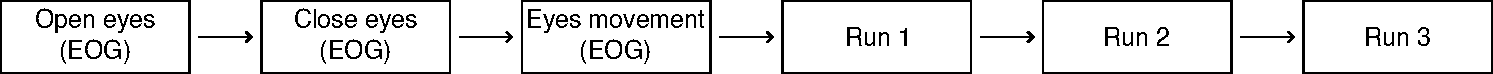
\includegraphics[width=\linewidth]{Figures/preliminaries/BCI2a_schema.pdf}
  \caption{Schema representing a one-day session of EEG data collection for the DBI MI \label{fig:bci2a_schema}}
\end{figure}

Subjects were instructed to sit on a comfortable armchair in front of a computer screen. \cref{fig:BCI2aprotocol} shows the seven-second MI protocol. The start was indicated by a short acoustic warning and a cross on a black screen for two seconds, then an arrow pointing left, right, down, or up indicated to the subjects to perform the desired MI task. Furthermore, the subjects were asked to continue the MI task until the cross disappeared \changes{three} seconds later. Afterward, a black screen indicated a short break until the beep and the cross reappeared, and a new trial started.

\begin{figure}[h!]
\centering
    \resizebox{0.5\linewidth}{!}{
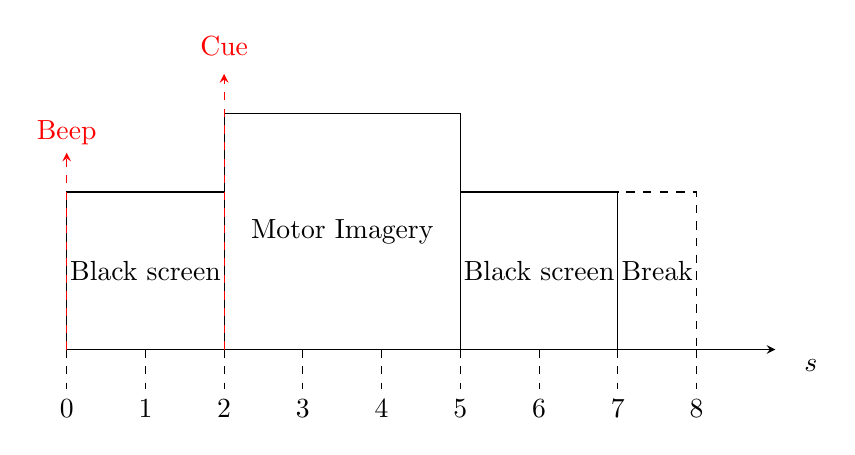
\begin{tikzpicture}
\draw[draw=black] (0,0) rectangle ++(2,2) node[pos=.5] {Black screen};
\draw[draw=black] (2,0) rectangle ++(3,3) node[pos=.5] {Motor Imagery};
\draw[draw=black] (5,0) rectangle ++(2,2) node[pos=.5] {Black screen};
\draw[dashed,draw=black] (7,0) rectangle ++(1,2) node[pos=.5] {Break};

% \draw[draw=red] (2.5,-0.2) rectangle ++(2,1) node[pos=.5] {\textcolor{red}{\small{Analysis span}}};
% \draw[dashed,draw=red] (2.5,0) -- (2.5,-1) node[pos=1.5] {\textcolor{red}{$2.5$}};
% \draw[dashed,draw=red] (4.5,0) -- (4.5,-1) node[pos=1.5] {\textcolor{red}{$4.5$}};

\draw [-stealth](0,0) -- (9,0) node[below,pos=1.05] {$s$};

\draw[dashed,draw=black] (0,0) -- (0,-0.5) node[pos=1.5] {$0$};
\draw[dashed,draw=black] (1,0) -- (1,-0.5) node[pos=1.5] {$1$};
\draw[dashed,draw=black] (2,0) -- (2,-0.5) node[pos=1.5] {$2$};

\draw[-stealth,dashed,draw=red] (2,0) -- (2,3.5) node[pos=1.1] {\textcolor{red}{Cue}};

\draw[-stealth,dashed,draw=red] (0,0) -- (0,2.5) node[pos=1.1] {\textcolor{red}{Beep}};

\draw[dashed,draw=black] (3,0) -- (3,-0.5) node[pos=1.5] {$3$};
\draw[dashed,draw=black] (4,0) -- (4,-0.5) node[pos=1.5] {$4$};
\draw[dashed,draw=black] (5,0) -- (5,-0.5) node[pos=1.5] {$5$};
\draw[dashed,draw=black] (6,0) -- (6,-0.5) node[pos=1.5] {$6$};
\draw[dashed,draw=black] (7,0) -- (7,-0.5) node[pos=1.5] {$7$};
\draw[dashed,draw=black] (8,0) -- (8,-0.5) node[pos=1.5] {$8$};
\end{tikzpicture}}
    \caption{Illustration of the seven-second DBI MI protocol used in the study. The protocol commences with a short acoustic warning and a cross shown on a screen for two seconds, followed by an arrow indicating the type of MI task to be performed. The black screen marks a brief break interval between tasks.
    \label{fig:BCI2aprotocol}}
\end{figure}

\subsubsection{Data Recording}

Twenty-two Ag/AgCI electrodes with an inter-electrode distance of 3.5cm and an international $10-20$ montage were used to acquire brain activity as shown in \cref{fig:montagebci2a}. All signals were monopolar recorded with the left mastoid electrode serving as a reference and the right one as ground. Activity was sampled at \changes{$250 s$} and bandpass filtered between \changes{$0.5 Hz$} and \changes{$100 Hz$}. The amplifier sensitivity was set to $100 \mu V$. Additionally, a notch filter centered at \changes{$50 Hz$} was applied to diminish electrical line noise. Moreover, three monopolar EOG channels were also included with the same specifications but with amplifier sensitivity set to $1mV$. This was done with the intention of subsequent artifact removal strategies. An expert visually inspected all EEG recordings to mark trials with high noise artifacts.

\begin{figure}[h!]
\centering
    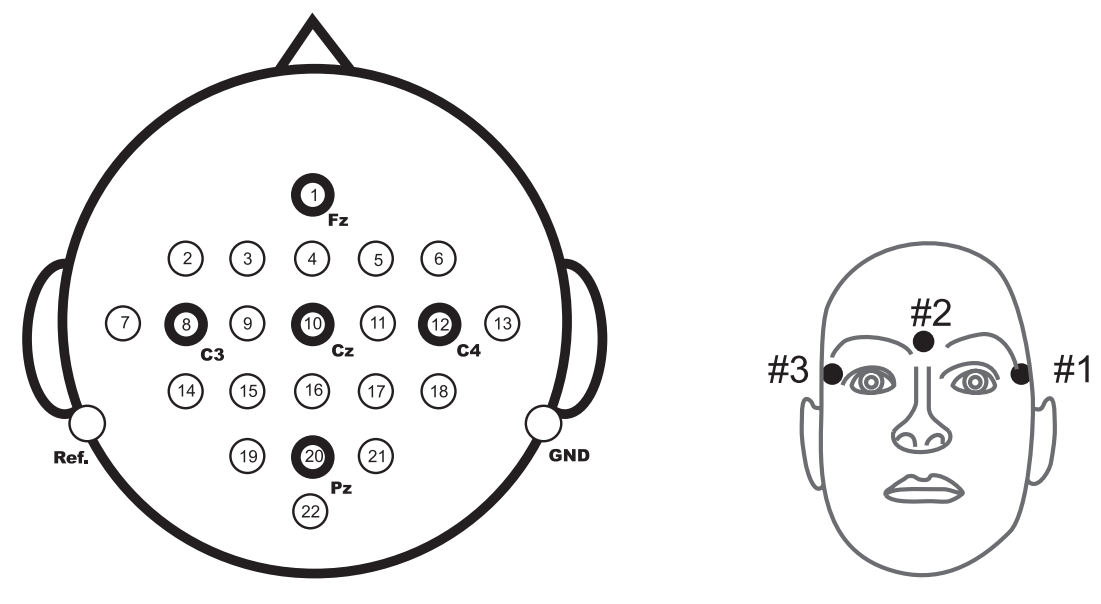
\includegraphics[width=0.6\linewidth]{Figures/preliminaries/bcielectrodes.PNG}
    \caption{Illustration of the electrode montage including the left image adhering to the international 10-20 system used for acquiring brain activity and the right image showing the montage of the three monopolar EOG channels employed for subsequent artifact removal. \textbf{Source:} \cite{brunner2008bci}. \label{fig:montagebci2a}}
\end{figure}

\subsection{Gamma Motor Execution Database---DBII ME}

\subsubsection{Protocol Design}

We explore the data that are publicly available at (\url{https://gin.g-node.org/robintibor/high-gamma-dataset}); this collection is a dataset collected by authors in \cite{schirrmeister2017deep}, obtained from $14$ healthy subjects ($6$ female, $2$ left-handed, age $27.2\pm 3.6$) with four-second trials of executed movements divided into $13$ runs per subject and ($R = 260$) trials were performed to collect each movement and rest. The four classes were movements of either the left hand, the right hand, both feet, and rest (no movement, but the same type of visual cue as the other classes). Visual cues were presented while using a monitor outside the cabin, which was visible through the shielded window. A fixation point was attached at the center of the screen. The subjects were instructed to relax, fixate on the mark, and keep as still as possible during the motor execution task. The tasks were as follows: Depending on the direction of a gray arrow that was shown on the black background. The subjects had to clench their toes (downward arrow), repetitively, perform sequential finger-tapping of their left (leftward arrow) or right (rightward arrow) hand, or relax (upward arrow). The movements were selected to require little proximal muscular activity while still being complex enough to keep subjects involved. Within the \changes{$4 s$} trials, the subjects performed the repetitive movements at their own pace, which had to be maintained as long as the arrow was showing. Per run, $80$ arrows were displayed for \changes{$4 s$} each, with $3$ to \changes{$4 Hz$} of continuous random inter-trial interval as shown in \cref{fig:gamma_time}

\begin{figure}[h!]
\centering
    \resizebox{1.0\linewidth}{!}{
\begin{tikzpicture}
\draw[draw=black] (0,0) rectangle ++(4,2) node[pos=.5] {Motor Execution $\#1$};
\draw[dashed,draw=black] (4,0) rectangle ++(4,2) node[pos=.5] {Random Break};
\draw[dashed,draw=black] (7,0) -- (7,2) node[pos=1.5] {};


% \draw[draw=red] (2.5,-0.2) rectangle ++(2,1) node[pos=.5] {\textcolor{red}{\small{Analysis span}}};
% \draw[dashed,draw=red] (2.5,0) -- (2.5,-1) node[pos=1.5] {\textcolor{red}{$2.5$}};
% \draw[dashed,draw=red] (4.5,0) -- (4.5,-1) node[pos=1.5] {\textcolor{red}{$4.5$}};

\draw [-stealth](0,0) -- (9,0) node[below,pos=1.05] {$s$};

\draw[dashed,draw=black] (0,0) -- (0,-0.5) node[pos=1.5] {$0$};

\draw[-stealth,dashed,draw=red] (0,0) -- (0,2.5) node[pos=1.1] {\textcolor{red}{Cue}};


\draw[dashed,draw=black] (4,0) -- (4,-0.5) node[pos=1.5] {$4$};

\draw[dashed,draw=black] (7,0) -- (7,-0.5) node[pos=1.5] {$7$};
\draw[dashed,draw=black] (8,0) -- (8,-0.5) node[pos=1.5] {$8$};


\end{tikzpicture}}
    \caption{Schema representing a one-run session of EEG data collection for the DBII ME
    \label{fig:gamma_time}}
\end{figure}

\subsubsection{Data Recording}

The EEG setup for the experiment comprised active electromagnetic shielding, high-resolution low-noise amplifiers, an actively shielded $128$-channel EEG cap, and full optical decoupling. All devices were battery-powered and communicated via optical fibers. Data were collected from $44$ sensors covering the motor cortex as shown in \cref{fig:eeg_gamma}, and were sampled at a rate of \changes{$500 Hz$}. Subjects were accommodated comfortably in a dimly lit Faraday cabin where they received visual cues on a monitor approximately $1$ meter away. A fixation point served as the focal point during the motor execution exercises. Subjects were instructed to stay still, relax, and limit body movements like blinking and swallowing to inter-trial intervals to ensure optimal data collection. The combined effect of the electromagnetic shielding and the comfortable, dimly lit environment helped maintain data coherence.

\begin{figure}[h!]
\centering
    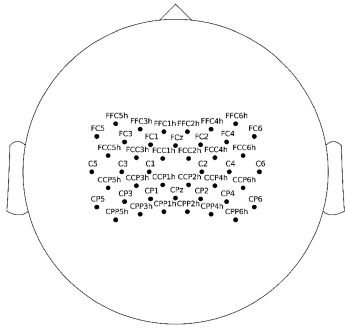
\includegraphics[width=0.4\linewidth]{Figures/preliminaries/gammaelectrodes.PNG}
    \caption{Positioning of the 44 sensors on the EEG cap, covering the motor cortex used for data collection in the motor execution experiment. Source: \cite{borra2019eeg} \label{fig:eeg_gamma}}
\end{figure}

\subsection{MI BCI EEG Giga Science Database - DBIII MI}

MI BCI EEG Giga Science database (DBIII MI) is an ideal choice for our validation as it has been widely used in the field of MI classification and has been shown to provide a robust benchmark for evaluating the performance of different models \cite{cho2017eeg}.
However, for the purpose of our study, we will only consider 50 subjects who met the minimum requirement of having at least 100 EEG trials recorded.

\subsubsection{Protocol Design}

This collection, publicly available at \footnote{\url{http://gigadb.org/dataset/100295}} and produced by researchers in \cite{cho2017eeg} holds EEG recordings obtained from 52 subjects ($M=52$), holding 19 females, performing two MI tasks ($N_y=2$) (left and right hand). $50$ were right-handed and $2$ left-handed. Data were gathered in a laboratory with a noise level between $37$ and $39$ decibels during one of the next time slots, T1 (9:30–12:00), T2 (12:30–15:00), T3 (15:30–18:00), or T4 (19:00–21:30).  $R=100$ trials of each label per subject were recorded by $C=64$ channels, where each channel was sampled at \changes{$512 Hz$}. Furthermore, EMG and EEG were recorded simultaneously with the same system and sampling rate to check actual hand movements.

\begin{figure}[h!]
\centering
    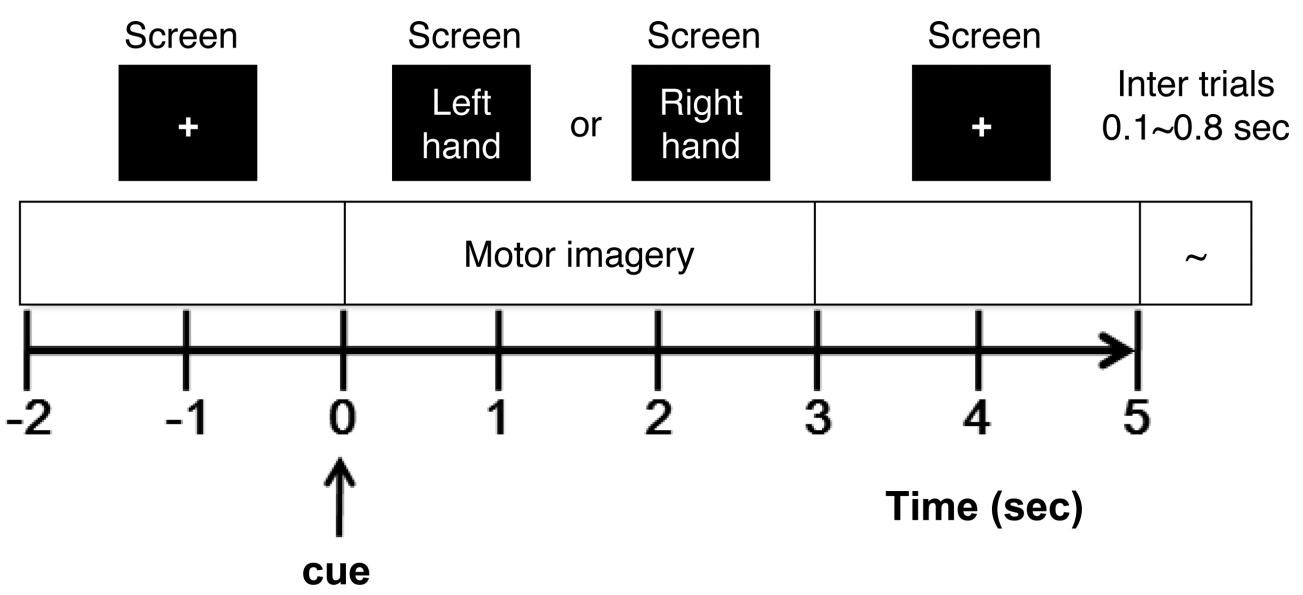
\includegraphics[width=0.7\linewidth]{Figures/preliminaries/protocol_giga.PNG}
    \caption{Diagram illustrating the experiment protocol involving motor imagery tasks. The figure shows the sequence of prompting, performing, and break periods in a single run. Source: \cite{cho2017eeg} \label{fig:protocol_giga}}
\end{figure}

The experiment involved non-motor related and motor imagery tasks, starting with data collected under six different types of noise conditions: eye blinking, eye movements, head movement, chewing, and resting state. Each noise type was recorded twice for five seconds, except for the resting state condition, which was recorded for 60 seconds. Following the noise data collection, subjects performed MI tasks, which were prompted via a monitor and conducted as per a protocol explained in \cref{fig:protocol_giga}. Each trial in this experiment stage started with a 2-second fixation on a cross displayed on a black screen. This was followed by a cue indicating a right or left-hand MI task. During the MI task, subjects were instructed to imagine the sensation of touching each finger of the designated hand with the thumb, beginning from the index finger and proceeding sequentially to the little finger. This emphasis on the kinesthetic rather than the visual aspect ensured that the subjects were indeed imagining the motor task. The MI task continued for 3 seconds, after which a blank screen signaled a rest period. This recovery interval lasted randomly between 2.1 and 2.8 seconds.

This task, break, and recovery cycle was repeated 20 times to form a complete run. Each subject performed between five and six such runs. After each run, a cognitive questionnaire was given to the subjects as an additional data collection point. Data quality was ensured by labeling and excluding trials with high voltage magnitude, classified as "bad trials", from the final analysis. Lastly, to maintain the engagement and motivation of the subjects, they were provided with feedback on the accuracy of their task performance after each run.



\subsubsection{Data Recording}

For this experiment, EEG data were collected using 64 active Ag/AgCl electrodes, according to a 64-channel montage based on the international 10-10 system and recorded at a sampling rate of \changes{$512 Hz$} as illustrated in Figure \ref{fig:dataset_sensors}. The Biosemi ActiveTwo system was employed for EEG collection, with instructions for left or right-hand motor imagery being presented through the BCI2000 system 3.0.2. EMG was recorded concurrently with EEG to verify actual hand movements, with two electrodes attached to the flexor digitorum profundus and extensor digitorum on each arm. For every participant, the EEG channel locations were recorded with a 3D coordinate digitizer; positions were averaged from three measurements to accommodate for possible hand tremors.

\begin{figure}[h!]
\centering
        \resizebox{0.4\linewidth}{!}{%% Creator: Inkscape 1.2.2 (b0a8486541, 2022-12-01), www.inkscape.org
%% PDF/EPS/PS + LaTeX output extension by Johan Engelen, 2010
%% Accompanies image file 'reference_plot_2.pdf' (pdf, eps, ps)
%%
%% To include the image in your LaTeX document, write
%%   \input{<filename>.pdf_tex}
%%  instead of
%%   \includegraphics{<filename>.pdf}
%% To scale the image, write
%%   \def\svgwidth{<desired width>}
%%   \input{<filename>.pdf_tex}
%%  instead of
%%   \includegraphics[width=<desired width>]{<filename>.pdf}
%%
%% Images with a different path to the parent latex file can
%% be accessed with the `import' package (which may need to be
%% installed) using
%%   \usepackage{import}
%% in the preamble, and then including the image with
%%   \import{<path to file>}{<filename>.pdf_tex}
%% Alternatively, one can specify
%%   \graphicspath{{<path to file>/}}
%% 
%% For more information, please see info/svg-inkscape on CTAN:
%%   http://tug.ctan.org/tex-archive/info/svg-inkscape
%%
\begingroup%
  \makeatletter%
  \providecommand\color[2][]{%
    \errmessage{(Inkscape) Color is used for the text in Inkscape, but the package 'color.sty' is not loaded}%
    \renewcommand\color[2][]{}%
  }%
  \providecommand\transparent[1]{%
    \errmessage{(Inkscape) Transparency is used (non-zero) for the text in Inkscape, but the package 'transparent.sty' is not loaded}%
    \renewcommand\transparent[1]{}%
  }%
  \providecommand\rotatebox[2]{#2}%
  \newcommand*\fsize{\dimexpr\f@size pt\relax}%
  \newcommand*\lineheight[1]{\fontsize{\fsize}{#1\fsize}\selectfont}%
  \ifx\svgwidth\undefined%
    \setlength{\unitlength}{558.00027682bp}%
    \ifx\svgscale\undefined%
      \relax%
    \else%
      \setlength{\unitlength}{\unitlength * \real{\svgscale}}%
    \fi%
  \else%
    \setlength{\unitlength}{\svgwidth}%
  \fi%
  \global\let\svgwidth\undefined%
  \global\let\svgscale\undefined%
  \makeatother%
  \begin{picture}(1,0.99999946)%
    \lineheight{1}%
    \setlength\tabcolsep{0pt}%
    \put(0,0){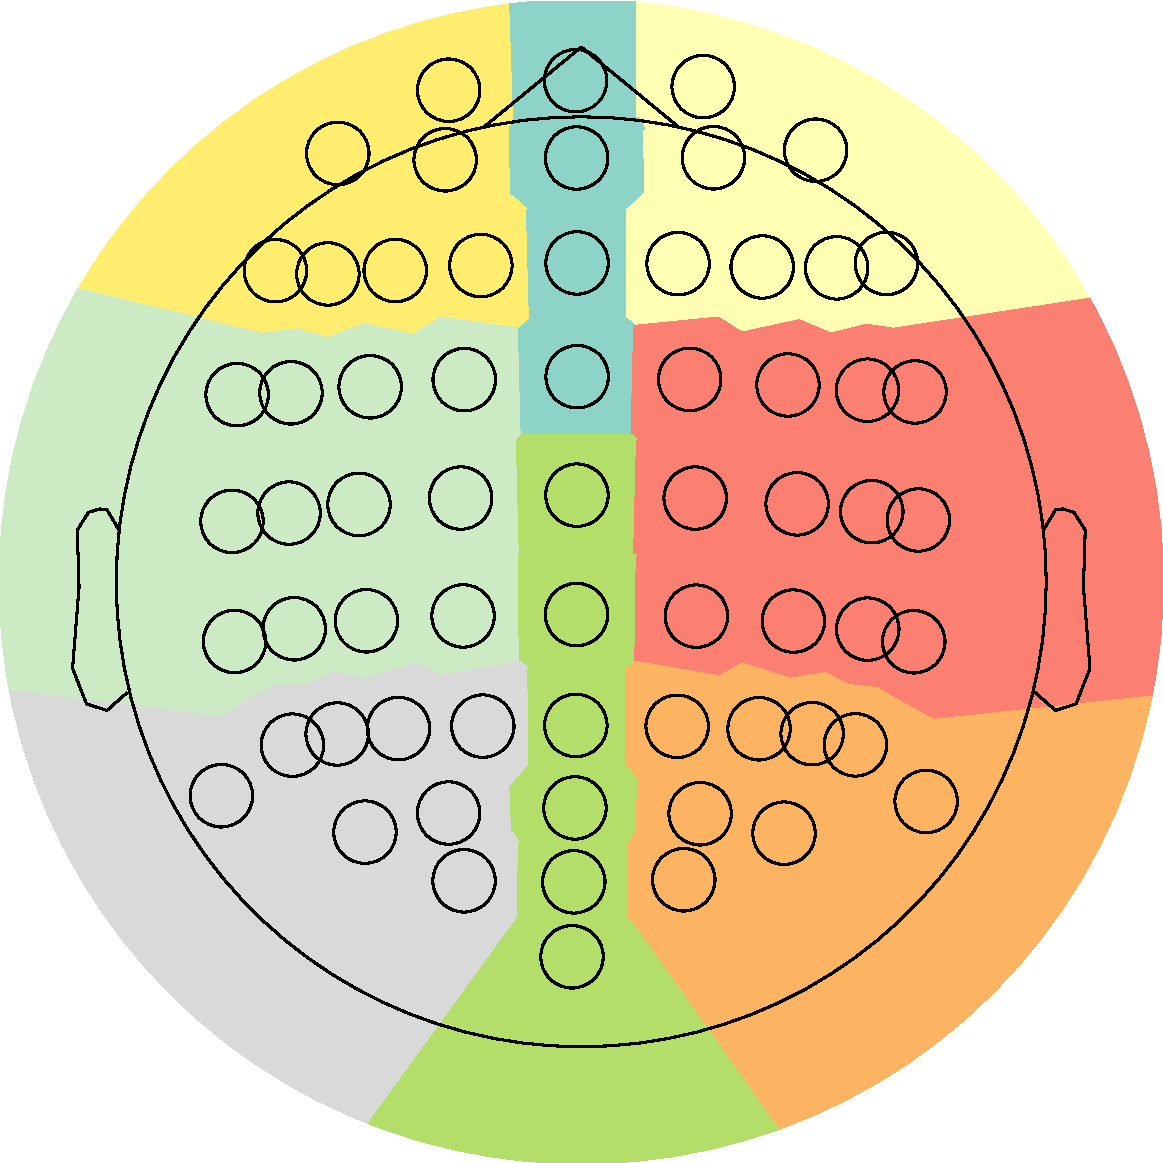
\includegraphics[width=\unitlength,page=1]{Figures/Objective_2/reference_plot_2.pdf}}%
    \put(0.36652085,0.91688558){\color[rgb]{0,0,0}\makebox(0,0)[lt]{\lineheight{1.25}\smash{\begin{tabular}[t]{l} \Large Fp1\end{tabular}}}}%
    \put(0.4768886,0.92508034){\color[rgb]{0,0,0}\makebox(0,0)[lt]{\lineheight{1.25}\smash{\begin{tabular}[t]{l} \Large Fpz\end{tabular}}}}%
    \put(0.58545766,0.9199935){\color[rgb]{0,0,0}\makebox(0,0)[lt]{\lineheight{1.25}\smash{\begin{tabular}[t]{l} \Large Fp2\end{tabular}}}}%
    \put(0.27059445,0.86251654){\color[rgb]{0,0,0}\makebox(0,0)[lt]{\lineheight{1.25}\smash{\begin{tabular}[t]{l} \Large AF7\end{tabular}}}}%
    \put(0.3629916,0.85707131){\color[rgb]{0,0,0}\makebox(0,0)[lt]{\lineheight{1.25}\smash{\begin{tabular}[t]{l} \Large AF3\end{tabular}}}}%
    \put(0.47724471,0.85857267){\color[rgb]{0,0,0}\makebox(0,0)[lt]{\lineheight{1.25}\smash{\begin{tabular}[t]{l} \Large AFz\end{tabular}}}}%
    \put(0.59373517,0.85882249){\color[rgb]{0,0,0}\makebox(0,0)[lt]{\lineheight{1.25}\smash{\begin{tabular}[t]{l} \Large AF4\end{tabular}}}}%
    \put(0.68165218,0.86525161){\color[rgb]{0,0,0}\makebox(0,0)[lt]{\lineheight{1.25}\smash{\begin{tabular}[t]{l} \Large AF8\end{tabular}}}}%
    \put(0.22412503,0.76166001){\color[rgb]{0,0,0}\makebox(0,0)[lt]{\lineheight{1.25}\smash{\begin{tabular}[t]{l} \Large F7\end{tabular}}}}%
    \put(0.26927017,0.7588327){\color[rgb]{0,0,0}\makebox(0,0)[lt]{\lineheight{1.25}\smash{\begin{tabular}[t]{l} \Large F5\end{tabular}}}}%
    \put(0.32722637,0.76178557){\color[rgb]{0,0,0}\makebox(0,0)[lt]{\lineheight{1.25}\smash{\begin{tabular}[t]{l} \Large F3\end{tabular}}}}%
    \put(0.40084017,0.76607436){\color[rgb]{0,0,0}\makebox(0,0)[lt]{\lineheight{1.25}\smash{\begin{tabular}[t]{l} \Large F1\end{tabular}}}}%
    \put(0.48479265,0.76828852){\color[rgb]{0,0,0}\makebox(0,0)[lt]{\lineheight{1.25}\smash{\begin{tabular}[t]{l} \Large Fz\end{tabular}}}}%
    \put(0.57052921,0.76768551){\color[rgb]{0,0,0}\makebox(0,0)[lt]{\lineheight{1.25}\smash{\begin{tabular}[t]{l} \Large F2\end{tabular}}}}%
    \put(0.64291322,0.76483078){\color[rgb]{0,0,0}\makebox(0,0)[lt]{\lineheight{1.25}\smash{\begin{tabular}[t]{l} \Large F4\end{tabular}}}}%
    \put(0.70693925,0.76411092){\color[rgb]{0,0,0}\makebox(0,0)[lt]{\lineheight{1.25}\smash{\begin{tabular}[t]{l} \Large F6\end{tabular}}}}%
    \put(0.74976654,0.7678815){\color[rgb]{0,0,0}\makebox(0,0)[lt]{\lineheight{1.25}\smash{\begin{tabular}[t]{l} \Large F8\end{tabular}}}}%
    \put(0.18501382,0.65500385){\color[rgb]{0,0,0}\makebox(0,0)[lt]{\lineheight{1.25}\smash{\begin{tabular}[t]{l} \Large FT7\end{tabular}}}}%
    \put(0.230178,0.65661815){\color[rgb]{0,0,0}\makebox(0,0)[lt]{\lineheight{1.25}\smash{\begin{tabular}[t]{l} \Large FC5\end{tabular}}}}%
    \put(0.29831107,0.66177952){\color[rgb]{0,0,0}\makebox(0,0)[lt]{\lineheight{1.25}\smash{\begin{tabular}[t]{l} \Large FC3\end{tabular}}}}%
    \put(0.37926054,0.6679257){\color[rgb]{0,0,0}\makebox(0,0)[lt]{\lineheight{1.25}\smash{\begin{tabular}[t]{l} \Large FC1\end{tabular}}}}%
    \put(0.47752226,0.67045104){\color[rgb]{0,0,0}\makebox(0,0)[lt]{\lineheight{1.25}\smash{\begin{tabular}[t]{l} \Large FCz\end{tabular}}}}%
    \put(0.57317084,0.66816088){\color[rgb]{0,0,0}\makebox(0,0)[lt]{\lineheight{1.25}\smash{\begin{tabular}[t]{l} \Large FC2\end{tabular}}}}%
    \put(0.65770736,0.66333128){\color[rgb]{0,0,0}\makebox(0,0)[lt]{\lineheight{1.25}\smash{\begin{tabular}[t]{l} \Large FC4\end{tabular}}}}%
    \put(0.72608603,0.65883651){\color[rgb]{0,0,0}\makebox(0,0)[lt]{\lineheight{1.25}\smash{\begin{tabular}[t]{l} \Large FC6\end{tabular}}}}%
    \put(0.76814418,0.65733992){\color[rgb]{0,0,0}\makebox(0,0)[lt]{\lineheight{1.25}\smash{\begin{tabular}[t]{l} \Large FT8\end{tabular}}}}%
    \put(0.18640365,0.54603203){\color[rgb]{0,0,0}\makebox(0,0)[lt]{\lineheight{1.25}\smash{\begin{tabular}[t]{l} \Large T7\end{tabular}}}}%
    \put(0.23460137,0.55313947){\color[rgb]{0,0,0}\makebox(0,0)[lt]{\lineheight{1.25}\smash{\begin{tabular}[t]{l} \Large C5\end{tabular}}}}%
    \put(0.29478238,0.56055995){\color[rgb]{0,0,0}\makebox(0,0)[lt]{\lineheight{1.25}\smash{\begin{tabular}[t]{l} \Large C3\end{tabular}}}}%
    \put(0.38224136,0.56605545){\color[rgb]{0,0,0}\makebox(0,0)[lt]{\lineheight{1.25}\smash{\begin{tabular}[t]{l} \Large C1\end{tabular}}}}%
    \put(0.48341184,0.56856097){\color[rgb]{0,0,0}\makebox(0,0)[lt]{\lineheight{1.25}\smash{\begin{tabular}[t]{l} \Large Cz\end{tabular}}}}%
    \put(0.58396329,0.56604577){\color[rgb]{0,0,0}\makebox(0,0)[lt]{\lineheight{1.25}\smash{\begin{tabular}[t]{l} \Large C2\end{tabular}}}}%
    \put(0.67165057,0.56107375){\color[rgb]{0,0,0}\makebox(0,0)[lt]{\lineheight{1.25}\smash{\begin{tabular}[t]{l} \Large C4\end{tabular}}}}%
    \put(0.73581692,0.55433585){\color[rgb]{0,0,0}\makebox(0,0)[lt]{\lineheight{1.25}\smash{\begin{tabular}[t]{l} \Large C6\end{tabular}}}}%
    \put(0.77680978,0.54719732){\color[rgb]{0,0,0}\makebox(0,0)[lt]{\lineheight{1.25}\smash{\begin{tabular}[t]{l} \Large T8\end{tabular}}}}%
    \put(0.18230964,0.44267411){\color[rgb]{0,0,0}\makebox(0,0)[lt]{\lineheight{1.25}\smash{\begin{tabular}[t]{l} \Large TP7\end{tabular}}}}%
    \put(0.23266377,0.45363629){\color[rgb]{0,0,0}\makebox(0,0)[lt]{\lineheight{1.25}\smash{\begin{tabular}[t]{l} \Large CP5\end{tabular}}}}%
    \put(0.29480849,0.46048839){\color[rgb]{0,0,0}\makebox(0,0)[lt]{\lineheight{1.25}\smash{\begin{tabular}[t]{l} \Large CP3\end{tabular}}}}%
    \put(0.37790608,0.46465505){\color[rgb]{0,0,0}\makebox(0,0)[lt]{\lineheight{1.25}\smash{\begin{tabular}[t]{l} \Large CP1\end{tabular}}}}%
    \put(0.47667086,0.46584238){\color[rgb]{0,0,0}\makebox(0,0)[lt]{\lineheight{1.25}\smash{\begin{tabular}[t]{l} \Large CPz\end{tabular}}}}%
    \put(0.57863054,0.46445265){\color[rgb]{0,0,0}\makebox(0,0)[lt]{\lineheight{1.25}\smash{\begin{tabular}[t]{l} \Large CP2\end{tabular}}}}%
    \put(0.66201097,0.46025166){\color[rgb]{0,0,0}\makebox(0,0)[lt]{\lineheight{1.25}\smash{\begin{tabular}[t]{l} \Large CP4\end{tabular}}}}%
    \put(0.7260133,0.45330943){\color[rgb]{0,0,0}\makebox(0,0)[lt]{\lineheight{1.25}\smash{\begin{tabular}[t]{l} \Large CP6\end{tabular}}}}%
    \put(0.76651151,0.442468){\color[rgb]{0,0,0}\makebox(0,0)[lt]{\lineheight{1.25}\smash{\begin{tabular}[t]{l} \Large TP8\end{tabular}}}}%
    \put(0.1773533,0.31000801){\color[rgb]{0,0,0}\makebox(0,0)[lt]{\lineheight{1.25}\smash{\begin{tabular}[t]{l} \Large P9\end{tabular}}}}%
    \put(0.23846259,0.35349394){\color[rgb]{0,0,0}\makebox(0,0)[lt]{\lineheight{1.25}\smash{\begin{tabular}[t]{l} \Large P7\end{tabular}}}}%
    \put(0.27698556,0.36310273){\color[rgb]{0,0,0}\makebox(0,0)[lt]{\lineheight{1.25}\smash{\begin{tabular}[t]{l} \Large P5\end{tabular}}}}%
    \put(0.32967442,0.36774008){\color[rgb]{0,0,0}\makebox(0,0)[lt]{\lineheight{1.25}\smash{\begin{tabular}[t]{l} \Large P3\end{tabular}}}}%
    \put(0.40221594,0.36989273){\color[rgb]{0,0,0}\makebox(0,0)[lt]{\lineheight{1.25}\smash{\begin{tabular}[t]{l} \Large P1\end{tabular}}}}%
    \put(0.48343935,0.37045952){\color[rgb]{0,0,0}\makebox(0,0)[lt]{\lineheight{1.25}\smash{\begin{tabular}[t]{l} \Large Pz\end{tabular}}}}%
    \put(0.56946187,0.36971499){\color[rgb]{0,0,0}\makebox(0,0)[lt]{\lineheight{1.25}\smash{\begin{tabular}[t]{l} \Large P2\end{tabular}}}}%
    \put(0.63988534,0.36763877){\color[rgb]{0,0,0}\makebox(0,0)[lt]{\lineheight{1.25}\smash{\begin{tabular}[t]{l} \Large P4\end{tabular}}}}%
    \put(0.68556707,0.36335775){\color[rgb]{0,0,0}\makebox(0,0)[lt]{\lineheight{1.25}\smash{\begin{tabular}[t]{l} \Large P6\end{tabular}}}}%
    \put(0.72274037,0.35377449){\color[rgb]{0,0,0}\makebox(0,0)[lt]{\lineheight{1.25}\smash{\begin{tabular}[t]{l} \Large P8\end{tabular}}}}%
    \put(0.7769358,0.3050661){\color[rgb]{0,0,0}\makebox(0,0)[lt]{\lineheight{1.25}\smash{\begin{tabular}[t]{l} \Large P10\end{tabular}}}}%
    \put(0.29258972,0.27868376){\color[rgb]{0,0,0}\makebox(0,0)[lt]{\lineheight{1.25}\smash{\begin{tabular}[t]{l} \Large PO7\end{tabular}}}}%
    \put(0.36456386,0.29509967){\color[rgb]{0,0,0}\makebox(0,0)[lt]{\lineheight{1.25}\smash{\begin{tabular}[t]{l} \Large PO3\end{tabular}}}}%
    \put(0.47439325,0.29952217){\color[rgb]{0,0,0}\makebox(0,0)[lt]{\lineheight{1.25}\smash{\begin{tabular}[t]{l} \Large POz\end{tabular}}}}%
    \put(0.58088867,0.29451737){\color[rgb]{0,0,0}\makebox(0,0)[lt]{\lineheight{1.25}\smash{\begin{tabular}[t]{l} \Large PO4\end{tabular}}}}%
    \put(0.65306662,0.27776523){\color[rgb]{0,0,0}\makebox(0,0)[lt]{\lineheight{1.25}\smash{\begin{tabular}[t]{l} \Large PO8\end{tabular}}}}%
    \put(0.38419722,0.23682676){\color[rgb]{0,0,0}\makebox(0,0)[lt]{\lineheight{1.25}\smash{\begin{tabular}[t]{l} \Large O1\end{tabular}}}}%
    \put(0.47975668,0.2359459){\color[rgb]{0,0,0}\makebox(0,0)[lt]{\lineheight{1.25}\smash{\begin{tabular}[t]{l} \Large Oz\end{tabular}}}}%
    \put(0.57316751,0.23772853){\color[rgb]{0,0,0}\makebox(0,0)[lt]{\lineheight{1.25}\smash{\begin{tabular}[t]{l} \Large O2\end{tabular}}}}%
    \put(0.48340759,0.17146872){\color[rgb]{0,0,0}\makebox(0,0)[lt]{\lineheight{1.25}\smash{\begin{tabular}[t]{l} \Large Iz\end{tabular}}}}%
  \end{picture}%
\endgroup%
}
    \caption{Sensor positions in a $10${--}$10$ placement electrode system, containing 64 channels. Besides, it highlights in color the main parts of the brain ( \legend{frontal_left} Frontal left, \legend{frontal} Frontal, \legend{frontal_right} Frontal right, \legend{central_right} Central right, \legend{posterior_right} Posterior right, \legend{posterior} Posterior, \legend{posterior_left} Posterior left, \legend{central_left} Central left)}
    \label{fig:dataset_sensors}
\end{figure}


\section{Theoretical Background}

In this section, we introduce the mathematical formulation of relevant related concepts used throughout this study.


\subsection{Motor Imagery Classification from EEG Signals}

\changes{MI involves the neural simulation of a movement that, although not physically executed, activates the same areas of the brain as actual movements. EEGs capture these activations, and machine learning models can be built to interpret these signals, allowing the prediction of human actions purely from the EEGs.}

\changes{From the mathematical perspective, let $\{\mat{X}_r\}_{r=1}^{R}$ be a multi-channel EEG observation from trial $r$, where each element $\mat{X}_r = \{\ve{x}_r^c  \in \Real^{N_t}\}_{c=1}^{N_c} $ contains $N_t \in \Natural$ time instants and $N_c \in \Natural$ number of channels. Moreover, there exists a function $\func{F}$ \eqref{eq:model} that exactly maps each trial $\mat{X}_r$ into the label space $y_r \in \{0, 1, \cdots, N_y\}$ representing the type of motor imagery with $N_y \in \Natural$ denoting the number of classes. The goal of EEG-MI classification is to find the best possible estimation function $\hat{\func{F}}(\cdot; \ve{w})$ that approximates the true function $\func{F}$ in \eqref{eq:model}, depending on a set of trainable parameters denoted as $\ve{w}$}

\begin{equation}\label{eq:model}
\func{F}: \mat{X}_r \mapsto y_r \quad \forall r \in \{1, \ldots, R\}    
\end{equation}



\subsubsection{Performance Measurement}

Performance measurement is necessary to evaluate the effectiveness of an EEG signal MI classification model. There are several commonly used metrics to measure the performance of such models, including Accuracy, Kappa coefficient, and the Area Under the Receiver Operating Characteristic Curve (AUC-ROC).

\textbf{Accuracy}: is the proportion of trials where a model correctly predicts the class label, represented as:

\begin{equation}
Acc = \frac{1}{R} \sum_{r=1}^{R} \Kronecker{\hat{y}_r}{y_r},
\end{equation}


where $\hat{y}_r$ and $y_r$ are the predicted and actual class labels, respectively, for the $r$-th trial, and $\Kronecker{\cdot}{\cdot}$ is the Kronecker delta function.

\textbf{Kappa Coefficient}: or Cohen’s kappa, measures inter-rater agreement. It considers the agreement occurring by chance, hence, providing a more robust metric than simple accuracy. Given a confusion matrix, the kappa coefficient can be calculated as:

\begin{equation}
\kappa = \frac{p_o - p_e}{1 - p_e}   , 
\end{equation}

where $p_o$ is the relative observed agreement, and $p_e$ is the hypothetical probability of random chance agreement.

\textbf{AUC-ROC curve}: AUC represents the probability that a classifier will rank a randomly chosen positive instance higher than a randomly chosen negative instance. The ROC curve is created by plotting the true positive rate (TPR) against the false positive rate (FPR) at various threshold settings.

For instance, let $\hat{p}_r$ be the predicted probability of the $r$-th trial belonging to the positive class. Then $\hat{p}_r = \sigma(\hat{\func{F}}(\mat{X}_r); \ve{w})$, where $\sigma(x) = 1/(1 + \exp(-x))$ is the logistic function that transforms the model output into a probability. Therefore, The TPR (or sensitivity) and FPR (or 1-specificity) can be defined as follows:

\changes{
\begin{equation}
    TPR = \frac{\text{TP}}{\text{P}} = \frac{\sum_{r=1}^{R} \Kronecker{\hat{y}r}{ y_r}\Kronecker{y_r}{1}}{\sum_{r=1}^{R} \Kronecker{y_r}{1}},    
\end{equation}
}

\changes{
\begin{equation}
    FPR = \frac{\text{FP}}{\text{N}} = \frac{\sum_{r=1}^{R} \Kronecker{\hat{y}_r}{ 1}\Kronecker{y_r}{0}}{\sum_{r=1}^{R} \Kronecker{y_r}{0}},
\end{equation}
}

where TP is the number of true positives, FP is the number of false positives, P is the number of positive instances, and N is the total number of negative ones. Thus, the AUC can be computed by integrating the curve over the interval $[0,1]$. In practice, the integral is estimated by the trapezoidal rule since we only have a finite number of instances from which to construct the ROC curve. In essence, the AUC-ROC measures the model's ability to discriminate positive from negative cases.

\subsection{Stochastic Processes}
\changes{A stochastic process, in the context of MI-BCI systems, serves as a robust mathematical construct for characterizing the progression of underlying random systems over distinct mental events. More specifically, $\ve{\chi}^{c}_{e}$ outlines the behavior of the $c$-th channel at an event $e$. A trial or sample $r$ of the event $e$ can be draw and be denoted as $x^c_{e, r}(\tau)$. This process characteristically encompasses a diverse array of random varibales that mimic the dynamism inherent within an event. Hence, a set $\{x^{c}_{er}(\tau)\}_{r=0, c=1}^{R, N_{c}}$ can effectively encapsulate the patterns within the stochastic process of the event $e$. For simplicity the notation $x^c_{r}(\tau)$ is used, assumming an specific event.
}

\subsubsection{Random Process Moments}
 
In the study of random processes, 'moments' are vital quantitative measures that describe data set features, including mean, variance, skewness, and kurtosis. In this context, the focus is on the first and second moments. \changes{The first moment is the mean}, providing a central data point while the second moment relates to the variance and correlation, indicating data dispersion and the relationship between variables, respectively. These moments give a comprehensive view of the dataset's structure and dynamics.

\subsubsection{First Moment}

The first moment, also known as the expectation, \changes{of a random variable $x^{c}_{r}(\tau)$}, represents the expected value or mean of the variable. It serves as a measure of the center of the data distribution. The expectation can be mathematically defined as follows:

\changes{
\begin{equation}
    \mathbb{E}_{\tau}\{x^{c}_{r}(\tau)\} = \mu^{c}_{r} = \int_{-\infty}^{+\infty} \tau P^{c}_{r}(\tau) d\tau,
\end{equation}
}

\changes{where $P^{c}_{r}(\tau)$ is the probability density function of the channel $c$ at trial $r$.}

\subsubsection{Second Moment}

The second moment of a random variable, often referred to as the variance, denoted as \changes{$\mathcal{\tilde{R}}^{c}_{r}$}, serves as the measure of how much the potential outcomes of the variable deviate from its mean value. This quantifies the spread or dispersion of the data. The formulation for variance can be computed as follows.
\changes{
\begin{equation}
  \begin{split}
    \mathcal{\tilde{R}}^{c}_{r}(\tau) = \mathbb{E}_{\tau}\{(x^{c}_{r}(\tau) - \mu^{c}_{r})^2\} &= \int_{-\infty}^{+\infty} \left( \tau-\mu^{c}_{r} \right) ^2 P^{c}_{r}(\tau) d\tau \\
    &= \mathbb{E}_{\tau}\{(x^{c}_{r}(\tau))^2\} - (\mathbb{E}\{x^{c}_{r}(\tau)\})^2
  \end{split}
\end{equation}
}
In the context of EEG-based MI-BCI systems, there is a common practice of centering each channel by eliminating the mean value. Consequently, when \changes{$\mu^{c}_{r}=0$}, the variance equation can be reformulated as:

\changes{
\begin{equation}
  \begin{split}
    \mathcal{\tilde{R}}^{c}_{r}(\tau) = \mathbb{E}_{\tau}\{(x^{c}_{r}(\tau))^2\} &= \int_{-\infty}^{+\infty}  (\tau)^2 P^{c}_{r}(\tau) d\tau \\
    &= \mathbb{E}_\tau\{(x^{c}_{r}(\tau))^2\}
  \end{split}
\end{equation}
}

The Covariance, another important concept intertwined with variance, measures the joint variability or spread of two random variables. It determines how much the variables change together and quantifies their dependency. \changes{If two channels ar trial $r$ $x^{c}_{r}$ and $x^{c'}_{r}$ are centered, $\mu^{c}_{r}=0$ and $\mu^{c'}_{r}=0$, the covariance $\mathcal{\tilde{R}}^{c, c'}_{r}$} can be computed as follows.

\changes{
\begin{equation}
  \begin{split}
    \mathcal{\tilde{R}}^{c, c'}_{r}(\tau) = \mathbb{E}_{\tau} \left[ x^{c}_{r}(\tau) x^{c'}_{r}(\tau)  \right] = \mathbb{E}_{\tau} \left[ x^{c'}_{r}(\tau) x^{c}_{r}(\tau) \right] \label{corr_est}
  \end{split}
\end{equation}
}

\changes{
Covariance is essential in many strategies, such as Common Spatial Patterns (CSP), used for MI-BCI, as they capture the relationships between different EEG channels $c$, and $c'$ at trial $r$.} These relationships contain relevant information regarding neuronal oscillations and synchronization, both of which are crucial aspects of MI tasks. 

\subsubsection{Wide/Weak-Sense Stationarity Stochastic Processes}

A stochastic process is deemed wide-sense stationary (WSS) or weak-sense stationary if it satisfies the following two conditions.

\begin{enumerate}
    \item The mean function or the first moment of the process is constant. This implies that the expected value or the average value of the process should be constant over time and not rely on the underlying time. Mathematically, it is represented by the equation:
    \changes{
    \begin{equation}
        \mathbb{E}_{\tau}\{x^{c}_{r}(\tau)\} = \mu^{c}_{r} = \text{constant, for all } \tau,
    \end{equation}
    where $\mathbb{E}_{\tau}\{x^{c}_{r}(\tau)\}$ denotes the expected value of the random variable at any time $\tau$ and $\mu^{c}_{r}$ is the constant mean value.}

    \item The autocorrelation function or the second moment of the process depends only on the difference in time and not the actual time. This suggests that the correlation between two variables taken at different periods should only depend on the difference between those periods. It can be mathematically expressed as follows.

    \changes{
    \begin{equation}
        \mathbb{E}_{\tau}\{(x^{c}_{r}(\tau_1)-\mu^{c}_{r})(x^{c}_{r}(\tau_2)-\mu^{c}_{r})\} = \mathcal{\tilde{R}}^{c}_{r}(\tau_1 - \tau_2) = \mathcal{\tilde{R}}^{c}_{r}(\tau_{\Delta}),
    \end{equation}
    Where the autocorrelation function $\mathcal{\tilde{R}}^{c}_{r}(\tau_1 - \tau_2) = \mathcal{\tilde{R}}^{c}_{r}(\tau_{\Delta})$ between two points at time instances $\tau_1$ and $\tau_2$ is only a function of their difference $\tau_{\Delta}=(\tau_2 - \tau_1)$.}
\end{enumerate}

\subsubsection{Wiener Khinchin Theorem}

According to the Wiener Khinchin theorem, the autocorrelation function \changes{$\mathcal{\tilde{R}}^{c}_{r}(\tau)$} of a WSS random process is a Fourier transform pair with its power spectral density \changes{$\tilde{P}^{c}_{r}[\omega]$}. This means that the autocorrelation function in the time domain corresponds to the power spectral density in the frequency domain and vice versa. This can be mathematically represented as follows.

\changes{
\begin{equation}
    \mathcal{\tilde{R}}^{c}_{r}(\tau) = \int_{\Real} \tilde{P}^{c}_{r}[\omega] e^{j 2\pi f \tau} df
\end{equation}
}

Likewise, the power spectral density is given by the Fourier transform of the autocorrelation function.

\changes{
\begin{equation}
    \tilde{P}^{c}_{r}[\omega] = \int_{\mathbb{f}} \mathcal{\tilde{R}}^{c}_{r}(\tau) e^{-j 2\pi f \tau} d\tau
\end{equation}
}

In the context of EEG-based MI-BCI systems, the Wiener-Khinchin theorem provides a useful tool for analyzing EEG signals. By transforming from the time domain to the frequency domain and vice versa, we gain insights into the spectral and temporal properties of the underlying stochastic processes, enabling efficient feature extraction and system identification.


\subsection{EEG Classical Feature Extraction Techniques}

The extraction of features from EEG signals is a crucial step towards decoding the information hidden within them. This step involves transforming the raw EEG data into a suitable set of features to represent the inherent properties that are key to differentiating different motor imagery classes. \changes{The random variable $x^{c}_{r}(\tau)$ is being discretize, usually at $250 Hz$ or $500 Hz$, creating a vector with $N_t$ time samples $\ve{x}^{c}_r \in \Real ^ {N_t}$. If all channels $N_c$ are concatenated the matrix $\mat{X}_{r} \in \Real^{N_c,N_t}$ can be constructed}. Let $\func{G}$ be a feature extraction function that transforms our raw EEG data into feature vectors as follows:
\begin{equation}
\ve{z}_r = \func{G}(\mat{X}_r),
\end{equation}

where $\ve{z}_r \in \Real^{N_p}$ represents the feature vector for trial $r$ with $N_p \in \Natural$ denoting the feature size. The feature extraction function $\func{G}$ can be defined in various ways based on different feature extraction methods. The objective here is to find an optimal feature extraction function $\func{G}$ such that the features $\ve{z}_r = \func{G}(\mat{X}_r)$ are discriminative enough for the classification of motor imagery EEG signals. After feature extraction step, the problem essentially becomes a feature-based classification problem, where we want to find a function $\hat{\func{F}}(\cdot,\ve{w})$ such that the estimated class label $\hat{y}_r = \hat{\func{F}}(\ve{z}_r; \ve{w})$ matches the true label $y_r$ as accurately as possible.

\subsubsection{Common Spatial Patterns}
\changes{
Common Spatial Pattern (CSP) is a widely used technique for extracting features from EEG signals, especially for MI tasks. CSP helps in identifying spatial filters that maximize the difference of variance between classes. the core concept of CSP is the simultaneous diagonalization of two covariance matrices. CSP relies on \cref{corr_est} to estimate the sample covariance matrix for each trial as follows:}

\changes{
\begin{equation}
   Cov(\mat{X}_r) = \mat{\Sigma}_{r} = \frac{1}{N_{t}-1} \mat{X}_r \mat{X}_{r}^T,
\end{equation}
}
\changes{
Where $Cov(\cdot)$ is the covariance fucntion, $\mat{\Sigma}_{r} \in \Real^{N_c \x N_c}$ is the covariance matrix for any trial $r$, $N_{t}$ is the number of time instances and $\mat{X}_{r}^{T}$ is the transpose of the EEG data matrix for trial $r$.
}
\changes{
Next, the average class covariance matrices $\Sigma_{C1}$ and $\Sigma_{C2}$ are calculated taking the sum of all covariance matrices for a class  divided by the total number of trials in that class. For instance, if we have a total of $R_{C1}$ trials in the set $C1$, the average clas matrix $\Sigma_{C1}$ can be computed as follows:
}
\changes{
\begin{equation}
\mat{\Sigma}_{C1} = \frac{1}{R_{C1}} \sum_{{r}=1}^{R_{C1}} \mat{\Sigma}_{r};\quad \forall r \in C1     
\end{equation}
}
A similar process can be followed to obtain the average covariance matrix for class $C2$.

The goal of CSP is to find a set of projection vectors (spatial filters) that could maximize the variance for one class while minimizing it for the other class as defined in \eqref{eq:CSP}.

\begin{equation}\label{eq:CSP}
\ve{w}^* = \max_{\ve{w}} \frac{\ve{w}^T \mat{\Sigma}_{C1} \ve{w}}{\ve{w}^T \mat{\Sigma}_{C2} \ve{w}}     
\end{equation}

The solution to this problem is given by the joint eigenvectors of $\mat{\Sigma}_{C1}$ and $\mat{\Sigma}_{C2}$ corresponding to the maximum and minimum eigenvalues. The transformed EEG is not directly used in classification models. Instead, a common approach is to use the log variance of the transformed signals and often take from the top and bottom few filters. First, compute the transformed signal as:

\begin{equation}
\mat{S}_r = \ve{w}^* \mat{X}_r     
\end{equation}

To calculate the final features for the CSP method, we compute the log variance of these transformed signals as follows:

\changes{
\begin{equation}\label{eq:CSPfeats}
\ve{z}_r = log \left( \frac{\diag{Cov({\mat{S}}_{r})}}{\Tr{Cov(\mat{S}_{r})}}  \right)  ,
\end{equation}
}
\changes{
Where $\Tr{\cdot}$ stands for the trace operator, $\diag{\cdot}$ is the diagonal operator that extracts the elements in the principal diagonal, and $log(\cdot)$ represent the element wise logarithmic operator}. For instance, if we're using CSP as our feature extraction method, $\func{G}_{CSP}$ will constitute the operations involved in \eqref{eq:CSPfeats}, where the filters corresponding to the highest and lowest eigenvalues are selected, such as the from $\ve{z}_r$ we take the first $N_p/2$ and last $N_p/2$ elements, where $N_p$ is the final desired number of features. Finally, these features $\ve{z}_r$ extracted by applying the CSP technique can now be fed to the classifier for further processing.

Sure, the requested sub-subsection would be as follows:

\subsubsection{Variations of Common Spatial Patterns}

Over time, various adaptations of the CSP method have been developed to address specific issues and improve performance. These include the next regularizations techniques weithtened by the $\alpha$ parameter:

\paragraph{Constant regularization:} Where a constant term is added to the sample variance for diminishing the risk of overfitting \cite{park2017filter}.

\changes{
\begin{equation}
    \hat{\mat{\Sigma}}=\{\mat{\Sigma}+\alpha \mathbf{I}\}
\end{equation}
}

\paragraph{Lasso regularization:} This method employs a penalty equal to the absolute value of the magnitude of the coefficients. It aims to simplify the used model by forcing some coefficients to zero in the spatial linear filters \cite{zhang2018new}.

\changes{
\begin{equation}
    \ve{w}^* = \max_{\ve{w}}\left( \frac{\ve{w}^T \mat{\Sigma}_{C1} \ve{w}}{\ve{w}^T \mat{\Sigma}_{C2} \ve{w}}  - \alpha\left\|\ve{w}\right\|_1\right)
\end{equation}
}

\paragraph{Tikhonov regularization:} A squared magnitude of the spatial filter coefficients is employed as a penalty term, preventing coefficients from reaching very high values that could lead to overfitting \cite{fauzi2019energy}

\changes{
\begin{equation}
    \ve{w}^* = \max_{\ve{w}}\left( \frac{\ve{w}^T \mat{\Sigma}_{C1} \ve{w}}{\ve{w}^T \mat{\Sigma}_{C2} \ve{w}} -  \alpha\left\|\ve{w}\right\|_2 \right)
\end{equation}
}

\paragraph{Elastic-net regularization:} This technique is a mix of the Lasso and Tikhonov regularizations, using both absolute and squared magnitudes, thus encompassing their benefits \cite{gu2021eeg}.

\changes{
\begin{equation}
    \ve{w}^* = \max_{\ve{w}}\left( \frac{\ve{w}^T \mat{\Sigma}_{C1} \ve{w}}{\ve{w}^T \mat{\Sigma}_{C2} \ve{w}}- \alpha\left\|\ve{w}\right\|_1 \frac{1-\alpha}{2} \left\|\ve{w}\right\|_2 \right)
\end{equation}
}

\paragraph{Weighted regularization:} The diagonal of the sample covariance matrix is penalized with distinct weights to differentially shrink their effect on the spatial filters.\cite{deng2020local}

\changes{
\begin{equation}
    \tilde{\mat{\Sigma}}=\{\mat{\Sigma}+\alpha\operatorname{diag}(\ve{a})\}
\end{equation}
}

\paragraph{Lq/p regularization:} A generalization of Lasso and Tikhonov regularizations. It is flexible with $q$ and $p$, which can be any non-negative real numbers, providing more control over the model complexity \cite{cai2021single}.

\changes{
\begin{equation}
    \ve{w}^* = \max_{\ve{w}}\left( \frac{\ve{w}^T \mat{\Sigma}_{C1} \ve{w}}{\ve{w}^T \mat{\Sigma}_{C2} \ve{w}}-\alpha\left\|\ve{w}\right\|_{p, q} \right)
\end{equation}
}

Each of these versions of CSP can be selected and implemented according to the specific demands and objectives of the dataset and problem at hand.

\subsubsection{Sub-band CSP}

In practice, EEG signals not only differ in spatial patterns but also in frequency bands. Sub-band Common Spatial Pattern (SBCSP) is an extension that considers the frequency components of the EEG signals. First, it decomposes the original EEG signals into various frequency bands before applying the CSP method to each band individually. The generated sub-band CSP features are then concatenated to create a more robust feature vector that includes both spatial and spectral information, resulting in improved performance in classifying motor imagery tasks.

Suppose we define a band-pass filter $\func{H}_f$ that decomposes an EEG signal into the frequency band $f \in \Omega$, where $\Omega$ is a set of filters. Thus, the filter operation can be represented as:

\begin{equation}
\tilde{\mat{X}}_{r,f} = \func{H}_f(\mat{X}_r)   , 
\end{equation}

where $\tilde{\mat{X}}_{r,q}$ represents the signal $\mat{X}_r$ in the frequency band $f$. Then, the CSP transformation is performed over the sub-band signals, and the variance of the transformed signals is used to construct the sub-band CSP features as follows:

\begin{equation}
\tilde{\ve{z}}_{r,f} = \func{G}_{CSP}(\tilde{\mat{X}}_{r,q}; \ve{w}_{f}^{*})   , 
\end{equation}

where $\func{G}_{CSP}$ is the function encapsulating the CSP featurization described in \eqref{eq:CSPfeats}, and $\ve{w}^{*}_{f}$ is the spatial filter for the frequency band $f$. Therefore, to obtain the complete feature vector $\ve{z}_r$ for trial $r$, the sub-band CSP features from all considered frequency bands are concatenated:

\begin{equation}
\ve{z}_r = [\tilde{\ve{z}}_{r,1}, \tilde{\ve{z}}_{r,2}, ..., \tilde{\ve{z}}_{r,N_f}]   ,
\end{equation}

where $N_f = \Cardinality{\Omega}$ is the total number of frequency bands and $\Cardinality{\cdot}$ stands or the set cardinality.

This method improves classification performance over the traditional CSP by incorporating frequency information. It better captures distinct patterns across different frequency bands to differentiate between motor imagery tasks.

\subsubsection{Time Windowing and Sub-Band CSP}

\changes{EEG signals often exhibit different patterns across different time intervals and frequency bands during a predefined mental taks}. Thus, along with the spatial and the frequency domain covered by sub-band CSP, it is also valuable to consider the time domain. We can incorporate information from the time dimension by applying a sliding time window over the continuous EEG signal and extracting sub-band CSP features from each time window. This way, we get a time-frequency (or t-f) distribution of CSP features, providing a more comprehensive representation of the signal for motor imagery classification tasks.

Suppose the raw EEG signal from trial $r$ is given by $\mat{X}_r$ and $\Delta_t$ be the time window set. Thus, we can split $\mat{X}_r$ into $\tau = \Cardinality{\Delta_t}$ time windows, each containing $N_{t}'$ time instants. $\mat{X}_{r,t} \in \Real^{N_c \x N_{t}'}$ denotes the signal in the $t$-th window. Next, we perform the sub-band CSP methods for each time-windowed signal. As a result, a sub-band CSP feature $\tilde{\ve{z}}_{r,t,f}$ for the $t$-th time window and $f$-th frequency band is obtained. Finally, to obtain the complete feature vector that incorporates time, frequency, and spatial information, we concatenate all the sub-band CSP features across all time windows and frequency bands as follows:

\begin{equation}
\ve{z}_r = [\tilde{\ve{z}}_{r,1,1}, \tilde{\mat{z}}_{r,1,2}, \cdots, \tilde{\ve{z}}_{r,\tau,N_f}]  .  
\end{equation}

This method is essentially an enhancement of the Sub-band CSP that considers the information encoded in the time, frequency, and spatial domains simultaneously. By viewing the time dimension, it extracts more comprehensive features, which can lead to improved classification performance on motor imagery tasks.


\subsection{Functional Connectivity Estimators}

In this section, we describe the most important functional connectivity estimators.

\subsubsection{Correlation}
Correlation (Corr) is a measure often used to represent the linear relationship between two EEG channels~\cite{fagerholm2020dynamic}. For two vectors $\ve{x}^{c}_{r}$ and $\ve{x}^{c'}_{r}$ from two channels $c$ and $c'$ at trial $r$ such that $c\neq c'$, the correlation is defined as:

\changes{
\begin{equation}
    Corr^{c, c'}_{r} =\frac{\mathbb{E}_{t}\left[\left(x^{c}_{r}[t]-\mu^{c}_{r}\right)\left(x^{c'}_{r}[t]-\mu^{c'}_{r}\right)\right]}{\sigma^{c}_{r} \sigma^{c'}_{r}},
\end{equation}
}

where $\mathbb{E}\{\cdot\}$ is the expected value, $\mu_{X^{c}}$ and $\mu_{X^{c'}}$ are the mean values and $\sigma_{X^{c}}$ and $\sigma_{X^{c'}}$ are the standard deviations of $X^{c}$ and $X^{c'}$ time series.

\changes{
\subsubsection{Cross-Correlation}
}
Cross-correlation (Cross-corr) differs from Corr since it is a function with respect to a time lag $\delta$, which can be expressed as follows \cite{roy2022comparative}.

\changes{
\begin{equation}
    \operatorname{Cross-corr}^{c,c'}_{r}(\delta)=\frac{\mathbb{E}_{t}\left[ \left( x^{c}_{r} [t] - \mu^{c} \right) \left(x^{c'}_{r}[t+\delta]-\mu^{c'}\right)\right]}{\sigma^{c} \sigma^{c'}}.
\end{equation}
}

\subsubsection{Magnitude Square Coherence}
The magnitude-squared coherence (MSC) is a measure that, as a function of frequency, estimates how well channel $c$ relates linearly to another channel $c'$~\cite{cattai2021phase}. \changes{It is defined by the squared modulus of the cross-spectrum $S^{c, c'}_{r}[\omega]$ of the two vectors, $\ve{x}^{c}_{r}$ and $\ve{x}^{c'}_{r}$, divided by the product of their auto-spectral densities $S^{c}_{r}[\omega]$ and $S^{c'}_{r}[\omega]$ as:
\begin{equation}
    MSC^{c,c'}_{r}[\omega] = \frac{|S^{c, c'}_{r}[\omega]|^2}{S^{c}_{r}[\omega]S^{c'}_{r}[\omega]}.
\end{equation}
}

\subsubsection{Phase Locking Value}

Phase Locking Value (PLV) is another technique commonly used in EEG analysis. PLV measures the consistency of the phase difference between a pair of channels, which can capture the synchronization activities between different brain regions. Suppose $x^{c}_{r}[t]$ is the EEG signal from channel $c$ at time $t$ and trial $r$. The instantaneous phase $\phi_{x^{c}}[t]$ can be extracted using the Hilbert transformation. \changes{According to authors in \cite{cattai2021phase}, the phase difference between channel $c$ and $c'$ is calculated as follows: 
}
\changes{
\begin{equation}
 \Delta \phi_{c,c'}[t] = \phi_{x^{c}}[t] - \phi_{x^{c'}}[t]    ,
\end{equation}
}
\changes{
hence, the PLV between the two channels is then computed by averaging the phase difference over the time dimension and taking the absolute value:}

\changes{
\begin{equation}
PLV^{c,c'}_{r}=\left| \frac {1}{N_t} \sum_{t=1}^{N_t} e^{j\Delta \phi_{c, c'}[t]} \right|    ,
\end{equation}
}
where $j$ is the imaginary unit, values range from $0$ to $1$, with $1$ indicating perfect phase locking (i.e., constant phase difference over time) and $0$ indicating a random phase relationship.

\subsubsection{Phase Lag Index}

The Phase Lag Index (PLI) captures the asymmetry of the distribution of phase differences between two signals and is calculated based on the relative phase difference between the two signals \cite{siviero2023functional}.

\changes{
\begin{equation}
    PLI^{c,c'}_{r} = |\mathbb{E}_t[\operatorname{sign}(\Delta \phi_{c,c'}[t])]|,
\end{equation}
}

The resulting value lies in the interval $[0,1]$, where a higher value indicates more phase synchrony.

\subsubsection{Weighted Phase Lag Index}
The Weighted Phase Lag Index (WPLI) is a measure of the phase synchronization between two signals~\cite{gonzalez2020network}. It's a modification of PLI but takes the magnitude of the imaginary component of cross-spectrum into account; thus, it is less sensitive to noise. This measure can be expressed mathematically by extending the PLI definition.

\changes{
\begin{equation}
    WPLI^{c, c'}_{r} = \frac{\left| \mathbb{E}_f \left[ \left| \Im[ S^{c, c'}_{r}[\omega] ] \right| \operatorname{sign}\left(\Im[ S^{c,c'}_{r}[\omega] ] \right) \right] \right|}{ \mathbb{E} \left[ \left| \Im[ S_{X^{c},X^{c'}} ] \right| \right]},
\end{equation}
where the $S^{c, c'}_{r}[\omega]$ is the cross-spectrum of signals in channels $c$ and $c'$ at trial $r$, $\Im[\cdot]$ denotes the imaginary part of a complex number, and$\operatorname{sign}(\cdot)$ denotes the sign function:
\begin{equation}
    \operatorname{sign}(x) = 
\begin{cases} 
1 & \text{if } x > 0, \\
0 & \text{if } x = 0, \\
-1 & \text{if } x < 0.
\end{cases}
\end{equation}
}

\subsubsection{Imaginary Part of the Coherence}

Imaginary Part of the Coherence (IPC) uses the imaginary part of the cross-spectrum, discarding any zero-lag interactions, often due to volume conduction, field spread, or common references \cite{cao2022brain}.
The IPC function can be derived from the cross-spectrum of two signals as follows.

\changes{
\begin{equation}
    IPC^{c, c'}_{r}[\omega] =  \frac{|\Im[S^{c, c'}_{r}[\omega]]|}{\sqrt{S^{c}_{r}[\omega]S^{c'}_{r}[\omega]}}
\end{equation}
}
\subsubsection{Partial Coherence}
Partial Coherence (PC) quantifies the unique linear relationship between two signals by removing the influence of other signals \cite{gonzalez2020network}. For multichannel signals, this can be understood as the coherence between two signals of interest after linearly regressing out the contributions from all other signals. 

\changes{
The PC between two signals $\ve{x}^{c}_{r}$ and $\ve{x}^{c}_{r}$ from two channels $c$ and $c'$ at trial $r$ can be represented as:
\begin{equation}
    PC^{c,c'}_{r}[\omega] = \frac{|S^{c, c'}_{r}[\omega]|^2 - |\sum_{k\neq c,c'}S^{c, k}_{r}[\omega]S^{c', k}_{r}[\omega]|^2}{(S^{c}[\omega]S^{c'}[\omega]) - (\sum_{k\neq c}S^{c, k}_{r}[\omega])^2 (\sum_{k\neq c'}S^{c', k}_{r}[\omega])^2},
\end{equation}
}
\changes{
where $S^{c, c'}_{r}[\omega]$ is the cross-spectrum between two signals $\ve{x}^{c}_{r}$ and $\ve{x}^{c'}_{r}$, $S^{c}_{r}[\omega]$ and $S^{c'}_{r}[\omega]$ are the power spectral densities of signals $\ve{x}^{c}_{r}$ and $\ve{x}^{c'}_{r}$ respectively. The sum is taken over all $k$ channels, excluding the channels $c$ and $c'$. 
}
\subsubsection{Mutual Information}

\changes{
According to information theory, the Mutual Information, $\operatorname{MI}$, of two random vectors $\ve{x}^{c}_{r}$ and $\ve{x}^{c'}_{r}$ shows how a random vector is informative for the other one. Let $P_{r}(\ve{x}^{c}_{r})$ and $P_{r}(\ve{x}^{c'}_{r})$ be the probability distributions of random vectors $\ve{x}^{c}_{r}$ and $\ve{x}^{c'}_{r}$ at trial $r$, respectively. The entropy of $\ve{x}^{c}_{r}$ and $\ve{x}^{c'}_{r}$ is defined as by \cite{gu2023decoding} as follows.}

\changes{
\begin{equation}
\begin{aligned}
& H(\ve{x}^{c}_{r})=-\sum_{t=0}^{N_t} P_{r}\left(x^{c}_{r}[t]\right) \log _{b}\left(P_{r}\left(x^{c}_{r}[t]\right)\right), \\
& H(\ve{x}^{c'}_{r})=-\sum_{t=0}^{N_t} P_{r}\left(x^{c'}_{r}[t]\right) \log _{b}\left(P_{r}\left(x^{c}_{r}[t]\right)\right),
\end{aligned}
\end{equation}
}

\changes{
where $t$ defines the time sample and $H(\ve{x}^{c}_{r} \mid \ve{x}^{c'}_{r})$ and $H(\ve{x}^{c}_{r}, \ve{x}^{c'}_{r})$ are conditional entropy and joint entropy between $X^{c}$ and $X^{c'}$, defined respectively as follows.
}

\changes{
\begin{equation}
\begin{aligned}
& H(\ve{x}^{c}_{r}, \ve{x}^{c'}_{r})=- \mathbb{E}_{\ve{x}^{c}_{r}}\left[ \mathbb{E}_{\ve{x}^{c'}_{r}}\left[\log _{b} P_{r}(\ve{x}^{c}_{r}, \ve{x}^{c'}_{r})\right]\right], \\
& H(\ve{x}^{c}_{r} \mid \ve{x}^{c'}_{r})=- \mathbb{E}_{\ve{x}^{c}_{r}}\left[ \mathbb{E}_{\ve{x}^{c'}_{r}}\left[\log _{b} P_{r}(\ve{x}^{c'}_{r} \mid \ve{x}^{c}_{r})\right]\right],
\end{aligned}
\end{equation}
}

\changes{
where $\mathbb{E}$ is the expected value function. MI of two random vectors $\ve{x}^{c}_{r}$ and $\ve{x}^{c'}_{r}$ is computed as 
\begin{equation}
\operatorname{MI}_{r}(\ve{x}^{c}_{r}, \ve{x}^{c'}_{r})=H(\ve{x}^{c}_{r})+H(\ve{x}^{c'}_{r})-H(\ve{x}^{c}_{r}, \ve{x}^{c'}_{r})=H(\ve{x}^{c'}_{r})-H(\ve{x}^{c'}_{r} \mid \ve{x}^{c}_{r})
\end{equation}
$\operatorname{MI}_{r}(\ve{x}^{c}_{r}, \ve{x}^{c'}_{r})=0$ if and only if random variables $\ve{x}^{c}_{r}$ and $\ve{x}^{c'}_{r}$ are statistically independent.
}
\subsubsection{Granger Causality}


Granger causality (GC) is a mathematical formalization of the Wiener's causality concept. \changes{For two stationary time series $\ve{x}^{c}$ and $\ve{x}^{c'}$, the linear autoregressive model is defined.
\begin{equation}
    x^{c'}_{r}[t] = \sum_{k=0}^{o} a_k x^{c'}_{r}[t-k] + \epsilon[t],
\end{equation}
Where $o$ is the model order, $a_k$ is the model coefficients, and $\epsilon[t]$ is the error at time $t$. 
}
Likewise, let define the bivariate autoregressive model as follows.

\changes{
\begin{equation}
     x^{c'}_{r}[t] = \sum_{k=0}^{o} a_k x^{c}_{r}[t-k] \sum_{k=0}^{o} b_k x^{c'}_{r}[t-k] + \epsilon'[t],
\end{equation}
}
where $o$ is the model order, $a_k$ and $b_k$ are the model coefficients, and $\epsilon'[t]$ is the error at time $t$. 

\changes{
The idea behind GC is that each value $x^{c'}_{r}[t]$ will be better defined including information from $x^{c}_{r}[t]$}, that means $|\ve{\epsilon'}|<|\ve{\epsilon}|$. Thus, the GC can be defined as follows \cite{rezaei2023classification}.

\changes{
\begin{equation} 
\operatorname{GC}(\ve{x}^{c}_{r} \rightarrow \ve{x}^{c'}_{r}) = \log \left( \frac{\operatorname{var}\{\ve{\epsilon}\}}{\operatorname{var}\{\ve{\epsilon'}\}} \right) ,
\end{equation}
}
where $\ve{\epsilon}, \ve{\epsilon'} \in \Real^{N_t-o}$ are vectors holding the \changes{prediction} errors, and $\operatorname{var}\{\cdot\}$ stands for the variance operator. If the past of \changes{$\ve{x}^{c}_{r}$} does not improve the prediction of \changes{$\ve{x}^{c'}_{r}$}, then $\operatorname{var}\{\ve{\epsilon}\} \approx \operatorname{var}\{\ve{\epsilon}'\}$ and \changes{$\operatorname{GC}(\ve{x}^{c}_{r} \rightarrow \ve{x}^{c'}_{r}) \rightarrow 0 $; if the prediction improves, then $\operatorname{var}\{\ve{\epsilon}\} \gg \operatorname{var}\{\ve{\epsilon}'\}$ and $\operatorname{GC}(\ve{x}^{c}_{r} \rightarrow \ve{x}^{c'}_{r}) \gg 0 $.}

\changes{\subsubsection{Directed Transfer Function}
The Directed Transfer Function (DTF) is based on the concept of Granger causality and estimated using multivariate autoregressive (MVAR) models, which uses all signals simultaneously \cite{rezaei2023classification}. First, the MVAR is calculated as follows:
\begin{equation}
    \mat{X}_{r}[t] = \sum_{t'=1}^{\tilde{p}} \left( \mat{A}_{r}[t'] \mat{X}_{r}[t-t'] \right) + \mat{\epsilon}[t],
\end{equation}
where $\mat{X}_{r}[t]$ is the matrix containing all channels at trial $r$ and time sample $t$, $\mat{A}_{r}[t']$ is the coefficient matrix at lag $t'$, $\tilde{p}$ is the model order, and $\mat{\epsilon}_{r}[t]$ is the residual matrix at time $t$ and trial $r$. Second, the MVAR model can be transformed into its frequency domain version using the Fourier transform to obtain the transfer fucntion matrix $\mat{H}_{r}[\omega]$ as follows:
\begin{equation}
    \mat{H}_{r}[\omega] = \left[ I - \sum_{t'=1}^{\tilde{p}}  \mat{A}_{r}[t'] \mathscr{F}\left( \mat{X}_{r}[t-t'] \right) \right]^{-1},
\end{equation}
where $\mat{H}_{r}[\omega]$ represents the transfer matrix, $\omega$ is the frequency and $\mathscr{F}$ is the Fourier transform. Finally, the influence from channel $c$ to channel $c'$ can be calculated as follows:
\begin{equation}
    \operatorname{DTF}^{c,c'}_{r}[\omega] = \frac{|h^{c,c'}_{r}[\omega]|^2}{\sum_{k=0}^{N_c} |h^{c,k}_{r}[\omega]|^2},
\end{equation}
where $h^{c,c'}_{r}{\omega}$ is the element of the transfer matrix $H_{r}[\omega]$ from channel $c$ to channel $c'$, and $N_c$ is the total number of cahnnels. The square of the magnitude of $h^{c,c'}_{r}[\omega]$ is normalized by the sum of squares of the magnitudes of all elements in channel $c$ of $H_{r}[\omega]$.
}

\subsubsection{Partial Directed Coherence}
\changes{
Partial Directed Coherence (PDC) is a frequency-domain measure based on MVAR models, designed to examine directed interactions between any pair of channels $c$ and $c'$. Similar to the DTF, the PDC is derived using Granger causality principles, but the normalization method differs, allowing the differenciation between direct and indirect interactions. As in DFT the first step is to fit the MVAR model to the data as follows:
\begin{equation}
    \mat{X}_{r}[t] = \sum_{t'=1}^{\tilde{p}} \left( \mat{A}_{r}[t'] \mat{X}_{r}[t-t'] \right) + \mat{\epsilon}[t],
\end{equation}
where $\mat{X}_{r}[t]$ is the matrix containing all channels at trial $r$ and time sample $t$, $\mat{A}_{r}[t']$ is the coefficient matrix at lag $t'$, $\tilde{p}$ is the model order, and $\mat{\epsilon}_{r}[t]$ is the residual matrix at time $t$ and trial $r$. Second, the MVAR model can be transformed into its frequency domain version using the Fourier transform to obtain the matrix of coefficient in the frequency  domain $\tilde{\mat{A}}_{r}[\omega]$ as follows:
\begin{equation}
    \begin{aligned}
    \tilde{a}^{c,c'}_{r}[\omega] &= \sum_{t'=0}^{\tilde{p}} \mathscr{F}\left( {a}^{c,c'}_{r}[t'] \right) ,\\
                                &= \sum_{t'=0}^{\tilde{p}} {a}^{c,c'}_{r}[t'] \exp^{j2\pi \omega \tau t'},
    \end{aligned}
\end{equation}
where $\tilde{a}^{c,c'}_{r}[0] = 1$, $\mat{H}_{r}[\omega]$ represents the transfer matrix, $\omega$ is the frequency and $\mathscr{F}$ is the Fourier transform. Finally, the PDC from channel $c$ to channel $c'$ at frequency $\omega$ and trial $r$ can be written as follows:
\begin{equation}
    \operatorname{PDC}^{c,c'}_{r}[\omega] =   \frac{\left|\tilde{a}^{c,c'}_{r}[\omega]\right|}{\sqrt{\left|\sum_{k=0}^{N_c}\tilde{a}^{c,k}_{r}[\omega]\right|^{2}}} .
\end{equation}
}

PDC ranges from $0$ to $1$, providing the degree of a direct influence of one channel on another in the frequency domain \cite{gaxiola2017using}.

\subsubsection{Transfer Entropy}

Transfer Entropy  (TE) is an alternative measure of direct functional connectivity based on information theory. TE does not require a model of the interaction and is inherently nonlinear. \changes{TE for two observed channels $\ve{x}^{c}_{r}$ and $\ve{x}^{c'}_{r}$ can be written as:
\begin{equation}
\resizebox{0.9\textwidth}{!}{$\operatorname{TE}(\ve{x}^{c}_{r} \rightarrow \ve{x}^{c'}_{r}) = \sum_{x^{c'}_{r}[t+u], \ve{x}^{c'}[t]^{d_{\ve{x}^{c'}_{r}}}, \ve{x}^{c}_{r}[t]^{d_{\ve{x}^{c}_{r}}}} P\left( x^{c'}_{r}[t+u], x^{c'}_{r}[t]^{d_{\ve{x}^{c'}_{r}}}, \ve{x}^{c}_{r}[t]^{d_{\ve{x}^{c}_{r}}} \right) \log \left( \frac{P\left( x^{c'}_{r}[t+u] \mid x^{c'}_{r}[t]^{d_{\ve{x}^{c'}_{r}}}, \ve{x}^{c}_{r}[t]^{d_{\ve{x}^{c}_{r}}} \right)}{P\left( x^{c'}_{r}[t+u] \mid x^{c'}_{r}[t]^{d_{\ve{x}^{c'}_{r}}} \right)} \right),
$}
\end{equation}
where $t$ is a time-index and $u$ denotes the prediction time. $x^{c'}_{r}[t]^{d_{\ve{x}^{c'}_{r}}}$ and $x^{c}_{r}[t]^{d_{\ve{x}^{c}_{r}}}$ are $d_{\ve{x}^{c'}_{r}}-$ and $d_{\ve{x}^{c}_{r}}-$ dimensional delay vectors \cite{rezaei2023classification}. Note that the probability density functions is unknown. Hence, the first step is to estimate it using methods like histograms \cite{choi2021detecting}, kernel estimates \cite{kuang2021measuring}, or K-nearest neighbors \cite{martinez2020can}.}

\subsubsection{Synchronization Likelihood}
The Synchronization Likelihood (SL) method is based on the concept of generalized synchronization and can be applied to both linear and nonlinear systems \cite{gonzalez2021network}. \changes{From each time sample $x^{c}_{r}[t]$ the embedded vectors $\ve{q}^{c}_{r}$ are calculated as follows:
\begin{equation}
\ve{q}^{c}_{r}[t] = \left[x^{c}_{r}[t], x^{c}_{r}[t+l], x^{c}_{r}[t+2l], \ldots ,x^{c}_{r}[t+(m-1)l]\right],
\end{equation}
where $m$ is the embedding dimension and $l$ is the lag. Then, for each vector $\ve{q}^{c}_{r}[t]$ a time-lag simmilarity probability $p^{c}_{r}[t]$ is computed using a predefined distance $\varepsilon$ as follows:
\begin{equation}
    p^{c}_{r}[t] = \frac{1}{2(\tau_{\Delta2}-\tau_{\Delta1})} \sum_{t'=1}^{N_t} \tilde{\Theta}\left( \varepsilon - \left<\ve{q}^{c}_{r}[t],\ve{q}^{c}_{r}[t']\right>_{2} \right),
\end{equation}
where $\left<\cdot\right>_{2}$ is the Euclidena distance, $\tilde{\Theta}\left(\cdot\right)$ is the Heaviside step function described in \cref{eq:Heaviside}, $\tau_{\Delta1}$ is the Theiler correction to avoid autocorrealtion noise, and $\tau_{\Delta2}$ is the length of the time window of interest.
\begin{equation}
    \tilde{\Theta}(x) =
    \begin{cases} \label{eq:Heaviside}
        0, & \text{if } x\leq< 0 \\
        1, & \text{if } x > 0.
    \end{cases}
\end{equation}
Each channel $c$ at time $t$ has a critical distance $\varepsilon^{c}_{r}[t]$, that can be determined assumming $p^{c}_{r}[t] = p_{\text{ref}}$ and $p_{\text{ref}} \ll 1$. Hence, the number of channels where the embedded vectors $\ve{q}^{c}_{r}[t]$ and $\ve{q}^{c}_{r}[t']$ are closer than the critical distance can be computed as follows:
\begin{equation}
    h_{r}[t,t'] = \sum_{c=1}^{N_c} \tilde{\Theta} \left( \varepsilon^{c}_{r}[t] - \left<\ve{q}^{c}_{r}[t],\ve{q}^{c}_{r}[t']\right>_{2} \right),
\end{equation}
where $h_{r}[t,t']$ shows the number of embedded vectors that are alike and is bounded by $0 \geq h_{r}[t,t'] \leq N_c$. We can now defined the synchronization likelihood $SL^{c}_{r}[t,t']$ for each channel $c$ at trial $r$ and at any time point pair $[t,t']$ as:
\begin{equation}
    SL^{c}_{r}[t,t'] =
    \begin{cases}
        \frac{h_{r}[t,t']-1}{N_c-1}, & \text{if } \left<\ve{q}^{c}_{r}[t],\ve{q}^{c}_{r}[t']\right>_{2} < \varepsilon^{c}_{r}[t]\\
        0, & \text{if } \left<\ve{q}^{c}_{r}[t],\ve{q}^{c}_{r}[t']\right>_{2} \geq \varepsilon^{c}_{r}[t],\\
    \end{cases}
\end{equation} 
we can now take the average over all $t'$ time samples to obtain $SL^{c}_{r}[t]$, which describes how strongly the channel $c$ at time $t$ on trial $r$ is synchronized to all other $N_c - 1$ channels. SL is bounded by $p_{\text{ref}} \geq SL^{c}_{r}[t] \leq 1$. If channel $c$ is uncorrelated with the other channels, then $SL^{c}_{r}[t] = p_{\text{ref}} $; whereas if it achieves maximal synchronization with all channels, then $SL^{c}_{r}[t]= 1$ \cite{gonzalez2021network}. Note that to compute the pair-wise connectivity, the SL analysis should be conducted for each pair of channels independently.
}

\subsection{Reproducing Kernel Hilbert Spaces for Machine Learning}

The central idea behind Reproducing Kernel Hilbert Spaces (RKHS) is to use the kernel function to map the input data into a high-dimensional feature space where learning problems become more tractable. In the context of EEG signal classification for motor imagery tasks, the raw EEG data often resides in a high-dimensional and complex space. Traditional linear models might struggle to capture the intricate relationships hidden within accurately. By mapping the raw data into an RKHS via a suitable kernel function, we can transform the complex problem into a simpler one, enabling more effective learning and prediction. Moreover, many kernel methods project data into RKHS implicitly, avoiding the actual high-dimensional mapping and the accompanying computational burden (referred to as the "kernel trick").

\subsubsection{Reproducing Kernel Hilbert Spaces}
\changes{
Let $\kappa(\cdot,\cdot)$ be a real-valued positive definite kernel, $\mathcal{H}$ a nonempty space, and $\phi(\cdot)$ be a function that maps any element in $\mathcal{X}$ to the $\mathcal{H}$ space. One can define a vector space by taking a linear combination of the form
\begin{equation}
    \phi\left(\cdot\right) = \sum_{i=1}^{N} \alpha_{i}\kappa\left(\cdot,x_{i}\right)
\end{equation}
where $N \in \mathbb{N}$, $\alpha_{i} \in \Real $, and $\left\{ x_i \in \mathcal{X}; \quad \forall i \right\}$. Thus, the dot product between $\phi$ and another function $\phi'$, defined as $\phi'\left(\cdot\right) = \sum_{j=1}^{N} \beta_{j}\kappa\left(\cdot,x_{j}\right)$, can be defined as follows:
\begin{equation}
    \begin{aligned}
        \left< \phi, \phi' \right>  &= \sum_{i=1}^{N}\sum_{j=1}^{N'} \alpha_{i}\beta_{j}\kappa\left(x_{i},x_{j}\right). \\    
                                    &= \sum_{j=1}^{N'} \beta_{j}\phi\left(x_{j}\right). \\    
                                    &= \sum_{i=1}^{N} \alpha_{i}\phi'\left(x_{i}\right).
    \end{aligned}
\end{equation}
The dot product  $\left< \cdot, \cdot \right>$ is bilinear and symmetric, as $ \left< \phi, \phi' \right> =  \left< \phi', \phi \right> $. Furthermore, it is positive definite as for any function $\phi$ we have:
\begin{equation}
    \left< \phi, \phi \right> \sum_{i,j=1}^{N} \alpha_{i}\alpha_{j}\kappa\left(x_{i},x_{j}\right) \geq 0.
\end{equation}
Finally, the dot product is equivalent to the $\kappa(\cdot,\cdot)$ function as $ \left< \kappa(\cdot,x), \phi \right> = f(x)$ and $\left< \kappa(\cdot,x), \kappa(\cdot,x') \right> = \kappa(x,x')$. By virtue of these properties, positive definite kernels $\kappa$ are also called RKHS.
In general, an RKHS can be defined as follows:
\begin{definition}[Reproducing Knerl Hilbert Space]
    Let $\mathcal{X}$ be a nonempty set and $\mathcal{H}$ a Hilbert space of functions $\phi: \mathcal{X} \rightarrow \mathcal{H}$. Then, $\mathcal{H}$ is called a reproducing kernel Hilbert space endowed with the dot product $\left< \cdot, \cdot\right>_{\mathcal{H}}$, and the norm $\left| \phi \right|_{\mathcal{H}} = \sqrt{\left< \phi, \phi\right>_{\mathcal{H}}}$, if there exists a bilinear function $\kappa: \mathcal{X} \times \mathcal{X} \rightarrow \Real$ with the following properties.
    \begin{itemize}
        \item $\kappa$ has the reproducing property $\left< \kappa(\cdot,x), \phi \right> = f(x) \quad \forall f \in \mathcal{H}$, in particular $\left< \kappa(\cdot,x), \kappa(\cdot,x') \right> = \kappa(x,x')$.
        \item $\kappa$ spans $\mathcal{H}$, i.e. $\mathcal{H} = \overline{span\left\{ \kappa\left( x,\cdot \right) | x \in \mathcal{X}\right\}}, where \overline{X} denotes the completion of the set X$.
        \item RKHS uniquely determines $\kappa$, since the symmetry property is not fulfilled as $\left< \kappa(\cdot,x), \kappa'(\cdot,x') \right> = \kappa(x,x')$ but $\left< \kappa'(\cdot,x), \kappa(\cdot,x') \right> = \kappa'(x,x')$, then $\kappa(x,x') \neq  \kappa'(x,x')$
    \end{itemize}
\end{definition}
}

\subsubsection{Bochner's Theorem}
\changes{
Bochner’s theorem relates a time stationary kernel $\kappa_{x}\left(\tau_{\Delta}\right) = \kappa\left( x\left(\tau_1\right), x\left(\tau_2\right) \right)$ with its cross-spectral counterpart $S_{x}(\varpi) $ via the Fourier Transform as defined in \cref{eq:bochner}.
\begin{linenomath*}
	\begin{equation}\label{eq:bochner}
		\kappa_{x}(\tau_{\Delta})= \int_{\mathscr{F}} \exp{(j2\pi \tau_{\Delta} \varpi)} S_{x}(\varpi)d{\varpi},
	\end{equation}
\end{linenomath*}
}
\begin{theorem}
Let $\kappa(x, y)=q(x-y)$ be a translation invariant kernel, real-valued and symmetric. Assume that $q$ is continuous. Then the two following are equivalent:

(i) $\kappa$ is positive definite.

(ii) There exists a positive and finite measure $\mu$ on $\mathbb{R}^{p}$ such that $q$ is the Fourier Transform of $\mu$, i.e. for all $x \in \mathbb{R}^{p}$

\begin{equation}
q(x)=  \int_{\mathbb{R}^{p}} \exp\left({-i u^{\top} x} \right) \mu(u) du
\end{equation}
\end{theorem}

In the realm of EEG-based MI-BCI systems, Bochner's theorem is a powerful analytical tool. It allows for the transformation of kernels from the time domain to the frequency domain when scrutinizing EEG signals. By providing a profound understanding of the spectral and temporal properties of the underlying stochastic processes, this theorem plays a significant role in unraveling the intricate patterns in EEG data for efficient feature extraction and precise identification of cognitive processes.

\subsection{Information Theoretic Learning from Kernel Matrices}
%%%%%%%%%%%%%%%%%%%%%%%%%%%%%%%%
Information Theoretic Learning (ITL) is a learning framework that harnesses information theory for supervised and unsupervised learning algorithms. Unlike traditional models that use Shannon-based entropy, ITL utilizes Renyi's $\alpha$-order entropy, a more generalized concept \cite{li2020fast}. Shannon entropy is defined as the expected information of the outcomes of a random variable. For a continuous random variable $X$, and using the linear averaging operator, Shannon entropy can be represented as $H(X)=\mathbb{E}\{I(X)\}=\int p(x) I(x) d x$, where $I(x)=-\log (p(x))$. However, the linear mean is only a specific instance of the averaging operator. In general, the expected value connected with a monotonous function $g(x)$, with inverse $g^{-1}(x)$, is denoted as $\mathbb{E}\{x\}=g^{-1}\left(\int p(x) g(x) d x\right)$. Thanks to the additivity postulate for independent events, the possible options for $g(x)$ fall into either $g(x)=c x$ or $g(x)=c 2^{(1-\alpha) x}$, as demonstrated in \cite{renyi1961measures}. The former leads to the linear mean and consequently the Shannon entropy, while the latter results in:

\begin{equation}\label{eq:renyiint}
    H_{\alpha}(X)=\frac{1}{1-\alpha} \log \left(\int p(x)^{\alpha} d x\right) 
\end{equation}

This equation relates to Renyi's $\alpha$ entropy where $\alpha \neq 1$ and $\alpha \geq 0$ \cite{principe2010information,renyi1961measures}. It includes Shannon's entropy definition when $\alpha \rightarrow 1$. In cases when one must estimate entropy from discrete data, the probability density function of a discrete random variable $X,\left\{x_{i}\right\}_{i=1}^{n} \subset \mathbb{R}^{d}$, the Parzen density estimator can approximate as $\hat{p}(x)=\frac{1}{n} \sum_{i=1}^{n} \kappa\left(x, x_{i}\right)$, where $\kappa(\cdot, \cdot) \in \mathbb{R}$ is a positive definite kernel function. For the case of $\alpha=2$, the Parzen approximation provides:

\changes{ 
\begin{equation}\label{eq:renyisum}
    \hat{H}_{2}(X)=-\log \left(\frac{1}{n^{2}} \sum_{i, j=1}^{n} \kappa_{\sqrt{2}\sigma}\left(x_{i}, x_{j}\right)\right),
\end{equation}
the information potential, the quantity inside the log function, correspond to the squared norm $\frac{1}{n} \sum_{i=1}^{n} \phi(x_{i})$, which by the law of large numbers converges to $\left|\mathbb{E}\left\{ X \right\}\right|^{2}$. The empirical estimatior used in \cref{eq:renyisum} links both Hilbert space representations and it can be rewritten using the terms of a Gram matrix $\mat{K}_{ij} = \kappa_{2\sigma}\left(x_{i}, x_{j}\right)$ as follows.
\begin{equation}\label{eq:renyi_kernel}
    \hat{H}_{2}(X)=-\log \left(\frac{1}{n^{2}}  \|\mat{K}\|_{F}^{2}\right)+C(\sigma),
\end{equation}
where $C(\sigma)$ is the normalization factor of the Parzen window, the Frobenius norm of the Gram matrix $\mat{K}$, defined as $\|\mat{K}\|_{F}^{2}=\operatorname{tr}(\mat{K K})$, and $\operatorname{tr}(\cdot)$ is the matrix trace.
}
\changes{The cross-inforamtion portential seeks to quantify the information contribution of each sample involved in a Parzen approximation and is directly related to Renyi's entropy by a strictly monotonic function \cite{giraldo2014measures}. Moreover, \cref{eq:renyi_kernel} is an entropy-like value possessing properties similar to Renyi's entropy without having to estimate probability distributions. Given a Gram matrix $\mat{K}$ with elements $k_{i j} = \kappa\left(x_{i}, x_{j}\right)$, a kernel-based formulation of Renyi's $\alpha$-order entropy can be outlined as follows:}
\begin{equation}
    H_{\alpha}(\mat{K})=\frac{1}{1-\alpha} \log \left(\operatorname{tr}\left(\mat{K}^{\alpha}\right)\right),    
\end{equation}
which holds that $\operatorname{tr}(\mat{K})=1$. The power $\alpha$ of $\mat{K}$ can be obtained using the spectral theorem \cite{giraldo2014measures}.

\subsection{EEG Deep Learning Techniques}

DL has brought remarkable developments in various fields, and EEG signal classification is no exception. It offers the advantage of automatic feature extraction, reducing the need for manual intervention, and often outperforms traditional machine learning classifiers. DL consists of multiple interconnected layers, that work together to predict a given input sample. They can be divided into discriminative, representative, and generative models.

\subsubsection{Discriminative Models in Deep Learning}

These models play a vital role in numerous machine-learning applications, largely due to their extraordinary effectiveness in predicting class labels given the input data. Generally, discriminative models concentrate on learning the conditional probability, $P(y|x)$. In other words, they aim to model the decision boundary between classes. We can categorize discriminative models based on their architecture in the following manner.

\paragraph{Multilayer Perceptron}

Traditional multilayer perceptrons (MLPs), also known as feed-forward neural networks, are the simplest type of artificial neural network. Comprising input, hidden, and output layers, their main goal is to transform the input data into meaningful outputs by adjusting the weights associated with the nodes via a learning algorithm \changes{\cite{amin2019deep}}. Mathematically, the output of each neuron in the neural network can be represented as follows:

\begin{equation}
h_i = \sigma \left( \sum_{j=1}^{N_h} w_{ji} x_j + b_i \right),
\end{equation}

where $x_j$ represents the inputs, $w_{ji}$ the weights, $b_i$ the bias, $h_i$ the $i$-th layer, and $N_h$ is the number of layers. The function $\sigma$ is a nonlinear activation function, which introduces non-linearity into the output of a neuron. This assists in learning complex non-linear patterns within the data. Specifically in the field of MI-BCI classification, $h_0$ is the flattened representation of $\ve{X}_r$, while $h_{N_h}$ is the final layer representing $\ve{z}_r$.

The output $\ve{z}_r$, serves as the input for a classification layer that generates predictions. For binary classification, a function such as a sigmoid could be utilized to constrain the output between $0$ and $1$. In situations involving multi-class classification problems, a softmax function is generally employed.

\paragraph{Convolutional Neural Networks}

A Convolutional Neural Network (CNN) is a specialized architecture that is particularly useful for handling grid-like data, such as a time series or an image. It often consists of convolutional, pooling, and fully connected layers. Its core concept is to apply a set of learnable filters or kernels to the input samples \changes{\cite{zhang2021adaptive}}. For instance, a filter $\mat{W}_f$ can be defined for a raw EEG input data $\mat{X}_r$ at trial $r$ to get its filtered version $\hat{\mat{X}}_r$ as follows:

\begin{equation}
\hat{\mat{X}}_{r,f} = \varphi(\mat{X}_r; \mat{W}_f)  ,
\end{equation}

where $\varphi(\cdot, \mat{W}_f)$ is a convolutional layer and $\mat{W}_f$ are trainable weights. In addition, if $\mat{W}_f$ is set, the CNN is called pooling layers and can perform down-sampling operations to provide an abstracted form of representation and to reduce the computational cost for subsequent layers. 

CNNs can learn to extract hierarchically organized features, where initial layers capture local and generic features (like edges in an image or short-term changes in an EEG signal), and deeper layers capture more global and task-specific features. Through backpropagation and gradient descent, a CNN is trained to optimize the weights of the kernels in the convolutional layers and the weights in the fully connected layers to improve classification performance. In the context of EEG signal classification, convolutional layers can be used to automatically and adaptively extract local and shift-invariant features, and the fully connected layers can learn to differentiate between different classes of motor imagery tasks.

\paragraph{Recurrent Neural Networks}

Recurrent Neural Networks (RNNs) are designed to use sequential information by performing the same task for every element in a sequence, with the output depending on the previous computations. Each neuron or unit in an RNN takes the current and previously received inputs into account to generate the output. Mathematically, the hidden state $h_t$ at time $t$ can be calculated as:

\begin{equation}
h_t = \sigma(\ve{w}_{h} \ve{h}_{t-1} + \ve{w}_x \ve{x}_{r,t} + \ve{b}_h)
\end{equation}

The output at time $t$ can be represented as:

\begin{equation}
y_t = \psi(\ve{w}_{y}\ve{h}_t + \ve{b}_y)
\end{equation}

Here, $\ve{w}_{h}, \ve{w}_{x}, \ve{w}_{y}$ represent the weight matrices, while $b_t$ denotes the bias terms. $\sigma$ refers to the activation function, while $\psi$ typically represents a softmax function utilized in multi-class classification problems. Due to the consideration of the temporal dynamic behavior of inputs by RNNs, they are extensively used in the processing of sequential data. Furthermore, RRN variants are discussed  below.

\textbf{Gated Recurrent Unit (GRU)} is a variant of the standard RNN that attempts to solve the vanishing gradients problem, making it more efficient in handling longer sequences. It introduces two types of gates: update gates and reset gates. The update gates determine the degree to which the previous state information is kept for the current state, while the reset gates control the amount of past information that is forgotten \changes{\cite{luo2018exploring}}. Mathematically, the GRU computations are implemented with the following equations:

\begin{equation}
u_t = \sigma(\ve{w}_{hu}\ve{h}_{t-1} + \ve{w}_{xu}\ve{x}_t + \ve{b}_u)
\end{equation}

\begin{equation}
r_t = \sigma(\ve{w}_{hr}\ve{h}_{t-1} + \ve{w}_{xr}\ve{x}_t + \ve{b}_r)
\end{equation}

\begin{equation}
\widetilde{h}_t = \tanh(\ve{w}_{h}\ve{h}_{t-1}\odot r_t + \ve{w}_{x}\ve{x}_t + \ve{b}_h)
\end{equation}

\begin{equation}
h_t = (1 - u_t) \odot h_{t-1} + u_t \odot \widetilde{h}_t
\end{equation}

In these equations, $u_t$ is the update gate, $r_t$ is the reset gate, and $\widetilde{h}_t$ is the candidate activation.

Like the GRU, \textbf{Long Short-Term Memory (LSTM)} is designed to address the vanishing gradient problem encountered in standard RNNs \changes{\cite{kumar2019brain}}. However, LSTMs have a more complex structure. An LSTM introduces a cell state and three gates: an input gate, a forget gate, and an output gate. This additional complexity allows for the modeling of longer context dependencies. The following equations mathematically represent the LSTM computations:

\begin{equation}
f_t = \sigma(\ve{w}_{hf}\ve{h}_{t-1} + \ve{w}_{xf}\ve{x}_t + \ve{b}_f)
\end{equation}

\begin{equation}
i_t = \sigma(\ve{w}_{hi}\ve{h}_{t-1} + \ve{w}_{xi}\ve{x}_t + \ve{b}_i)
\end{equation}

\begin{equation}
\widetilde{C}_t = \tanh(\ve{w}_{hC}\ve{h}_{t-1} + \ve{w}_{xC}\ve{x}_t + \ve{b}_C)
\end{equation}

\begin{equation}
C_t = f_t \odot C_{t-1} + i_t \odot \widetilde{C}_t
\end{equation}

\begin{equation}
o_t = \sigma(\ve{w}_{ho}\ve{h}_{t-1} + \ve{w}_{xo}\ve{x}_t + \ve{b}_o)
\end{equation}

\begin{equation}
h_t = o_t \odot \tanh(C_t)
\end{equation}

In these equations, $f_t$, $i_t$, and $o_t$ correspond to the forget gate, input gate, and output gate, respectively, while $C_t$ denotes the cell state and $h_t$ is the hidden state.

\paragraph{Graph Neural Networks}

Graph Neural Networks (GNNs) represent an innovative shift in neural network architectures, emphasizing the relationships between data rather than treating each data point individually or with a set grid. GNNs are specifically designed for processing graphical data, providing an insightful approach to problems where data are represented as graphs, such as social networks, molecular chemistry, and brain connectivity networks \changes{\cite{ju2023graph}}. The fundamental idea in GNNs is the propagation and transformation of features through the vertices of a graph, where the feature of a given vertex is iteratively updated by aggregating features from its neighbors, similar to CNNs. The aggregation function is a critical design choice and can vary significantly per the specific GNN type. The aggregated features are then combined with the original features through a combining function, and a non-linear transformation is typically applied. 

Let us consider Graph Convolutional Networks (GCNs) as an example. In a GCN, the feature representation of each node, $\ve{H}^{(l)} \in \mathbb{R}^{n \times d}$, is updated in every layer $l \in \{0, \ldots, L\}$ by passing through the following propagation rule:

\begin{equation}
\ve{H}^{(l+1)} = \sigma\left(\widetilde{\ve{D}}^{-1/2}\widetilde{\ve{A}}\widetilde{\ve{D}}^{-1/2} \ve{H}^{(l)}\ve{W}^{(l)}\right),
\end{equation}

Where $\widetilde{\ve{A}} = \ve{A} + \ve{I}_N $ is the adjacency matrix of the undirected graph $G$ with added self-connections by including the identity matrix $\ve{I}_N$. $\widetilde{D}$ is the diagonal node degree matrix of $\widetilde{\ve{A}}$. $\ve{W}^{(l)}$ is the weight matrix for the $l$-th neural network layer, and $\sigma(\cdot)$ represents a non-linear activation function such as the ReLU. Thus, each node aggregates the features from its neighboring nodes defined by $\widetilde{\ve{A}}$. This creates a form of information exchange among adjacent nodes. Then, the linear transformation $\ve{W}^{(l)}$ is applied, following which it undergoes a non-linear activation function \changes{\cite{raeisi2022graph}}.

Other types of GNNs include Graph Attention Networks (GATs), which introduce an attention mechanism allowing different weights for different nodes in the neighborhood according to their relative importance \changes{\cite{demir2022eeg}}. \changes{While Graph Neural Networks are capable of managing complex graph-structured data, they can be computationally demanding due to the necessity of processing all nodes and their neighbors within the graph. However, ongoing advancements in optimization techniques are continually improving their efficiency \cite{gao2024graph}.}

\subsubsection{EEG-based Deep Learning MI Classification Models}

\paragraph{EEGnet:} is a compact CNN specifically designed for EEG-based BCIs proposed in \cite{lawhern2018eegnet}. It is versatile across various BCI paradigms, can be trained with limited data, and produces interpretable features. The network involves sequenced convolutional steps and utilizes depthwise separable convolutions to reduce the number of parameters that need training, thereby lowering the network's complexity. EEGNet effectively extracts temporal and spatial features and applies batch normalization before the Exponential Linear Unit (ELU) nonlinearity \changes{\cite{qiumei2019improved}}. Dropout and average pooling techniques are used to prevent over-fitting and dimension reduction, respectively. Interestingly, the model eliminates using a dense layer prior to the softmax classification to reduce free parameters; the architecture can be seen in \cref{table:eegnet}. This innovative approach ensures EEGNet's efficacy in capturing significant and diverse time-scale data and enhances the network's accuracy in EEG signal classification.

\begin{table}[h!]
\caption{EEGnet arquitecture}\label{table:eegnet}
\centering
\begin{tabular}{l|c|c|c|c}
\hline
\textbf{Layer} & \textbf{Filters} & \textbf{Kernel size} & \textbf{Stride} & \textbf{Extra parameters}\\
\hline
Conv2D & 8 & (1,32) & (1,1) & bias=False, padding=same\\ 
BatchNormalization & $\cdot$ & $\cdot$ & $\cdot$ & momentum=0.99, epsilon=0.001\\ 
\hline
DepthwiseConv2D & 16 & ($N_c$,1) & (1,1) & bias=False, $D_m= 2$ , max norm = 1  \\ 
BatchNormalization & $\cdot$ & $\cdot$ & $\cdot$ & momentum=0.99, epsilon=0.001\\ 
Elu & $\cdot$ & $\cdot$ & $\cdot$ & $\cdot$\\ 
AveragePooling2D & $\cdot$ & (1,4) & (1,1) & $\cdot$ \\ 
Dropout & $\cdot$ & $\cdot$ & $\cdot$ & $D_p = 0.5$\\
\hline
SeparableConv2D & 16 & (1,16) & (1,1) & bias=False, padding=same\\
BatchNormalization & $\cdot$ & $\cdot$ & $\cdot$ & momentum=0.99, epsilon=0.001\\
Elu & $\cdot$ & $\cdot$ & $\cdot$& $\cdot$\\
AveragePooling2D & $\cdot$ &(1,8) & (1,1)& $\cdot$\\
Dropout & $\cdot$ & $\cdot$ & $\cdot$ & $D_p = 0.5$\\
\hline
Flatten & $\cdot$ & $\cdot$ & $\cdot$ & $\cdot$\\
Dense & $\cdot$ & $\cdot$ & $\cdot$ & units=$N_y$\\
Softmax & $\cdot$ & $\cdot$ & $\cdot$ & $\cdot$\\
\hline
\end{tabular}
\end{table}

\paragraph{Shallowconvnet:} is a convolutional neural network (ConvNet) architecture designed specifically for EEG decoding tasks~\cite{schirrmeister2017deep}. It comprises two main convolutional layers where the first layer is intended to bandpass each EEG channel. Bandpass filtering is a critical process in EEG signal processing that serves to filter unwanted frequency components and retain frequencies of interest. The second layer of the ShallowConvNet operates similar to spatial filters that process the signals in the spatial domain. An average pooling layer is applied in the ShallowConvNet to reduce spatial data and dimensionality, thereby helping curb overfitting. To further mimic the filter bank common spatial pattern (FBCSP) strategy~\cite{ang2008filter}, a broadly accepted approach in building spatial filters for EEG signal classification, a fully connected layer is added to the ShallowConvNet. The activation function used in this model is both square and logarithmic in nature, which aims to introduce non-linearity to the model and help it learn complex patterns. The architecture can be seen in \cref{table:shallownet}

\begin{table}[h!]
\caption{Shallowconvnet architecture}\label{table:shallownet}
\centering
\begin{tabular}{l|c|c|c|c}
\hline
\textbf{Layer} & \textbf{Filters} & \textbf{Kernel size} & \textbf{Stride} & \textbf{Extra parameters}\\
\hline
Conv2D & 40 & (1,13) & (1,1)&max norm = 2 \\
Conv2D & 40 & ($N_c$,1) & (1,1)&max norm = 2 \\
BatchNormalization & $\cdot$ & $\cdot$ & $\cdot$ & momentum=0.99, epsilon=0.001\\ 
Square activation & $\cdot$ & $\cdot$ & $\cdot$ & $\cdot$\\
AveragePooling2D & $\cdot$ &(1,35) & (1,7)& $\cdot$\\
log activation & $\cdot$ & $\cdot$ & $\cdot$ & $\cdot$\\
Dropout & $\cdot$ & $\cdot$ & $\cdot$ & $D_p = 0.5$\\
\hline
Flatten & $\cdot$ & $\cdot$ & $\cdot$ & $\cdot$\\
Dense & $\cdot$ & $\cdot$ & $\cdot$ & units=$N_y$\\
Softmax & $\cdot$ & $\cdot$ & $\cdot$ & $\cdot$\\
\hline
\end{tabular}
\end{table}

\paragraph{Deepconvnet:} also introduced by~\cite{schirrmeister2017deep}, is built to glean deeper, more intricate features by implementing additional convolutional layers. This model goes beyond the two-layer structure of the ShallowConvNet, incorporating three more convolutional layers, thus creating a five-layer network structure. While this model's complexity possibly aids in unearthing subtle patterns or features not discernible with less sophisticated models, it also poses potential risks. Due to its complexity, DeepConvNet is more susceptible to overfitting, where it could end up learning not the underlying patterns for different neural states but rather, specific variability present in individual trials. As such, when utilizing DeepConvNet, particular care must be taken to monitor and prevent overfitting, which might involve techniques such as regularization or early stopping. The architecture can be seen in \cref{table:deepconvnet}

\begin{table}[h!]
\caption{Deepconvnet architecture}\label{table:deepconvnet}
\centering
\begin{tabular}{l|c|c|c|c}
\hline
\textbf{Layer} & \textbf{Filters} & \textbf{Kernel size} & \textbf{Stride} & \textbf{Extra parameters}\\
\hline
Conv2D & 25 & (1,5) & (1,1)&max norm = 2 \\
Conv2D & 25 & ($N_c$,1) & (1,1)&max norm = 2 \\
BatchNormalization & $\cdot$ & $\cdot$ & $\cdot$ & momentum=0.1, epsilon=1e-5\\ 
Elu & $\cdot$ & $\cdot$ & $\cdot$ & $\cdot$\\
MaxPooling2D & $\cdot$ &(1,2) & (1,2)& $\cdot$\\
Dropout & $\cdot$ & $\cdot$ & $\cdot$ & $D_p = 0.5$\\
\hline
Conv2D & 50 & (1,5) & (1,1)&max norm = 2 \\
BatchNormalization & $\cdot$ & $\cdot$ & $\cdot$ & momentum=0.1, epsilon=1e-5\\ 
Elu & $\cdot$ & $\cdot$ & $\cdot$ & $\cdot$\\
MaxPooling2D & $\cdot$ &(1,2) & (1,2)& $\cdot$\\
Dropout & $\cdot$ & $\cdot$ & $\cdot$ & $D_p = 0.5$\\
\hline
Conv2D & 100 & (1,5) & (1,1)&max norm = 2 \\
BatchNormalization & $\cdot$ & $\cdot$ & $\cdot$ & momentum=0.1, epsilon=1e-5\\ 
Elu & $\cdot$ & $\cdot$ & $\cdot$ & $\cdot$\\
MaxPooling2D & $\cdot$ &(1,2) & (1,2)& $\cdot$\\
Dropout & $\cdot$ & $\cdot$ & $\cdot$ & $D_p = 0.5$\\
\hline
Conv2D & 200 & (1,5) & (1,1)&max norm = 2 \\
BatchNormalization & $\cdot$ & $\cdot$ & $\cdot$ & momentum=0.1, epsilon=1e-5\\ 
Elu & $\cdot$ & $\cdot$ & $\cdot$ & $\cdot$\\
MaxPooling2D & $\cdot$ &(1,2) & (1,2)& $\cdot$\\
Dropout & $\cdot$ & $\cdot$ & $\cdot$ & $D_p = 0.5$\\
\hline
Flatten & $\cdot$ & $\cdot$ & $\cdot$ & $\cdot$\\
Dense & $\cdot$ & $\cdot$ & $\cdot$ & units=$N_y$\\
Softmax & $\cdot$ & $\cdot$ & $\cdot$ & $\cdot$\\
\hline
\end{tabular}
\end{table}

\paragraph{TCNet-Fusion:} is a more recent approach proposed by~\cite{musallam2021electroencephalography} that comprises three main parts. Like EEGnet, it includes a temporal component that allows for learning different bandpass frequencies and a depth-wise separable convolution to extract spatial features for each temporal filter. A Temporal Convolutional Network (TCN) block is also applied to extract temporal patterns, which are then concatenated with the output of a separable convolution to alleviate feature loss. These outputs are then flattened and concatenated, followed by a separable convolution. A final dense layer with softmax activation is used to classify the concatenated features into MI classes. Similarly, adversarial learning has been successfully applied in many DL applications; these architectures rely on training a generative model that enforces invariance and generalization. Regardless, adversarial architectures are affected by overfitting, especially with subjects that do not have a similar pattern in each session \cite{ozdenizci2019adversarial}. The architecture can be seen in \cref{table:tcfnet}

\begin{table}[h!]
\caption{TCNet-Fusion architecture}\label{table:tcfnet}
\centering
\begin{tabular}{l|c|c|c|c}
\hline
\textbf{Layer} & \textbf{Filters} & \textbf{Kernel size} & \textbf{Stride} & \textbf{Extra parameters}\\
\hline
Permute & $\cdot$ & $\cdot$ & $\cdot$ & (2,1,3)\\
Conv2D & 24 & (32,1) & (1,1) & bias=False, padding=same \\
BatchNormalization & $\cdot$ & $\cdot$ & $\cdot$ & momentum=0.99, epsilon=0.001\\ 
\hline
DepthwiseConv2D & 16 & (1, $N_c$) & (1,1) & bias=False, $D_m= 2$ , max norm = 1  \\ 
BatchNormalization & $\cdot$ & $\cdot$ & $\cdot$ & momentum=0.99, epsilon=0.001\\ 
Elu & $\cdot$ & $\cdot$ & $\cdot$ & $\cdot$\\ 
AveragePooling2D & $\cdot$ & (8,1) & (1,1) & $\cdot$ \\ 
Dropout & $\cdot$ & $\cdot$ & $\cdot$ & $D_p = 0.5$\\
\hline
SeparableConv2D & 48 & (16,1) & (1,1) & bias=False, padding=same\\
BatchNormalization & $\cdot$ & $\cdot$ & $\cdot$ & momentum=0.99, epsilon=0.001\\
Elu & $\cdot$ & $\cdot$ & $\cdot$& $\cdot$\\
AveragePooling2D & $\cdot$ &(8,1) & (1,1)& $\cdot$\\
Dropout-2 & $\cdot$ & $\cdot$ & $\cdot$ & $D_p = 0.5$\\
\hline
TCN-Blocks $\cdot$ & $\cdot$ & $\cdot$ & $\cdot$ & layers=$2$, kernel-s=$4$, filt=$12$ $D_p$=$0.3$, N-residuals=2 \\
Concatenate $\cdot$ & $\cdot$ & $\cdot$ & $\cdot$ & [TCN-blocks, Dropout-2] \\
\hline
Flatten-1 $\cdot$ & $\cdot$ & $\cdot$ & $\cdot$ & [Dropout-2] \\
Flatten-2 $\cdot$ & $\cdot$ & $\cdot$ & $\cdot$ &  [Concatenate] \\
Concatenate $\cdot$ & $\cdot$ & $\cdot$ & $\cdot$ & [Flatten-1, Flatten-2] \\
\hline
Dense & $\cdot$ & $\cdot$ & $\cdot$ & units=$N_y$\\
Softmax & $\cdot$ & $\cdot$ & $\cdot$ & $\cdot$\\
\hline
\end{tabular}
\end{table}

\subsection{Explainable AI in MI-BCI}

Explainable Artificial Intelligence (XAI) is a rapidly evolving field that aims to make the decision-making process of complex AI models understandable. In the context of MI-BCI, XAI can provide valuable insights into how predictions are made, thereby enhancing trustworthiness, causality, transferability, confidence, fairness, accessibility, and interactivity \cite{arrieta2020explainable}. XAI techniques can be categorized based on interpretation types, model specificity, explanation scopes, and explanation forms. 

Regarding interpretation types, we have intrinsic and post-hoc techniques. Intrinsic techniques provide an explanation based on the structure or components of the model itself. For instance, in linear regression models, the trained weights can provide an intrinsic interpretation, indicating the contribution of each feature. On the other hand, post-hoc techniques refer to external methods that analyze a trained model, such as Class Activation Maps (CAMs).

In terms of model specificity, we have model-specific and model-agnostic techniques. Model-specific techniques require a unique model structure or property. Therefore, all intrinsic models fall into this category as they rely on the model structure \cite{tjoa2020survey}. Model-agnostic techniques, on the other hand, do not have any special requirements for the model, making them widely used in XAI models.

Explanation scope can be either global or local. Local explanations focus on the variables that contribute to the decision for a single input, providing insights into the main characteristics associated with that input. Global explanations aim to give insights into the model itself, explaining the interactions of the model parameters and answering the question of how the model makes predictions.

Finally, explanation forms can be divided into feature-based and example-based explanations. Feature-based explanations use gradient or feature map values to approximate the input importance, highlighting the parts that impact the final decision the most. An overlay map over the original input sample commonly represents them. Example-based explanations, on the other hand, try to explain models by showing one or more examples similar to the given input, usually extracted at the training step.

\subsubsection{Class Activation Maps}

Class Activation Maps (CAMs) are powerful visualization tools that highlight the input regions important for making predictions in Convolutional Neural Networks (CNNs). They provide a heatmap visualization that indicates the areas in the input image that the model focuses on when making a prediction. CAMs are based on the concept that the spatial information is encoded in the feature maps of convolutional layers in CNNs. By projecting the weights of the output layer back onto the convolutional feature maps, we can generate a coarse heatmap for each class in the output layer. This heatmap, or CAM, indicates the discriminative image regions CNN uses to identify a specific class.

The CAM for a particular class $c$ can be computed as follows:

\begin{equation}
    L_{CAM} = \sum_k w_{k,c} F_k,
\end{equation}

where $F_k$ are the spatial feature maps of the last convolutional layer, and $w_{k,c}$ are the weights corresponding to class $c$ in the output layer. The CAM $M_c$ is a weighted combination of the feature maps, where the weights are determined by the importance of the feature map for class $c$.

\subsubsection{Gradient Class Activation Maps}

Gradient Class Activation Maps (Grad-CAMs) are an extension of CAMs that aim to provide visual explanations of decisions made by any Convolutional Neural Network (CNN) architecture without requiring any re-training or modification to the original model. Grad-CAMs use the gradient information flowing into the last convolutional layer of the CNN to understand each neuron for a decision of interest. These gradients, flowing backward from the specific class at the output, are global-average-pooled to obtain the neuron importance weights. These are then used to create a coarse localization map highlighting the important regions in the image for predicting the concept.

The Grad-CAM for a particular class $c$ is computed as follows:

\begin{equation}
    L_{Grad-CAM}^c = ReLU\left(\sum_k \alpha_k^c F_k\right),
\end{equation}

where $F_k$ are the spatial feature maps of the last convolutional layer, and $\alpha_k^c$ are the neuron importance weights for class $c$, computed as the global average of the gradients of the class score with respect to the feature map. The $ReLU(\cdot)$ function ensures that only the features that positively influence the class of interest are visualized.

\subsubsection{Layer Class Activation Maps}

Layer Class Activation Maps (Layer CAM) is a recent advancement in the field of explainable AI, providing a method to visualize the regions of input that are important for making predictions in Convolutional Neural Networks (CNNs). Layer CAM extends the concept of CAMs and Grad-CAMs by offering a more precise localization of the important regions. Layer CAM leverages the gradient information of the last convolutional layer to generate a heatmap that highlights the discriminative regions in the input image. Unlike Grad-CAM, which uses global average pooling of gradients, Layer CAM directly multiplies the feature maps with the corresponding gradients, followed by a $ReLU$ operation and a channel-wise summation to generate the final heatmap.

The Layer CAM for a particular class $c$ is computed as follows:

\begin{equation}
    L_{Layer-CAM}^c = ReLU\left(\sum_k F_k \cdot \frac{\partial y^c}{\partial F_k}\right),
\end{equation}

where $F_k$ are the spatial feature maps of the last convolutional layer, and $\frac{\partial y^c}{\partial F_k}$ are the gradients of the class score concerning the feature map. The $ReLU(\cdot)$ function ensures that only the features that positively influence the class of interest are visualized.

\section{Computing Resources}
The experiments were carried out on Python-based libraries, including the well-known Scikitlearn, TensorFlow, and Keras. We have used the free tier of Google Colaboratory and Kaggle cloud computing services with the following specifications. 

\begin{itemize}
    \item \textbf{Google Colaboratory\footnote{\url{https://colab.research.google.com/}}:} provides 2 CPU cores, approximately 12 Gb of RAM, and 12/16 Gb on GPU
    \item \textbf{Kaggle\footnote{\url{https://www.kaggle.com/}}:} provides 4 CPU cores, 16Gb RAM and 16Gb on GPU
\end{itemize}

In addition, the research group has as a regional ally the Centro de Bioinformática y Biología Computacional - BIOS, which provides a computer specialized in machine learning with a 32-core processor, 500Gb of RAM, and a 16Gb GPU.